% CS-323 AI CEP report. Build: tectonic main.tex  (copy main.pdf to ../CS24045.pdf)
\documentclass[11pt]{article}
% !TEX root = main.tex
% Format rules (spec §8.2, REQ-RPT-11): Times New Roman, 11 pt body, 12 or 14 pt headings.

\usepackage{iftex}
\ifXeTeX
  % Tectonic / XeLaTeX: the real Times New Roman if installed (ttf-ms-fonts on Arch);
  % otherwise TeX Gyre Termes, a Times clone shipped with every TeX bundle.
  \usepackage{fontspec}
  \IfFontExistsTF{Times New Roman}
    {\setmainfont{Times New Roman}}
    {\setmainfont{TeX Gyre Termes}%
     \typeout{WARNING: Times New Roman not found, using TeX Gyre Termes}}
\else
  % Overleaf with pdfLaTeX: Times clone.
  \usepackage[T1]{fontenc}
  \usepackage{newtxtext}
\fi
\usepackage{amsmath,amssymb}

\usepackage[a4paper,margin=2.2cm]{geometry}
\usepackage{graphicx}
\graphicspath{{figures/}{../figures/}{../screenshots/}}
\usepackage{pdfpages}
\usepackage{booktabs}
\usepackage{tabularx}
\usepackage{float}
\usepackage{caption}
\captionsetup{font=small,labelfont=bf}
\usepackage{enumitem}
\setlist{itemsep=1pt,topsep=3pt}
\usepackage{algorithm}
\usepackage{algpseudocode}
\usepackage{xcolor}
\usepackage[hidelinks]{hyperref}

% Headings: 14 pt sections, 12 pt subsections (REQ-RPT-11).
\usepackage{titlesec}
\titleformat{\section}{\fontsize{14}{17}\selectfont\bfseries}{\thesection.}{0.5em}{}
\titleformat{\subsection}{\fontsize{12}{14}\selectfont\bfseries}{\thesubsection}{0.5em}{}
\titlespacing*{\section}{0pt}{10pt}{4pt}
\titlespacing*{\subsection}{0pt}{8pt}{3pt}

% Page numbers in the footer; the rubric page (page 1) has none.
\usepackage{fancyhdr}
\pagestyle{fancy}
\fancyhf{}
\fancyfoot[C]{\thepage}
\renewcommand{\headrulewidth}{0pt}

\setlength{\parindent}{0pt}
\setlength{\parskip}{4pt}

\newcommand{\astar}{A\textsuperscript{*}}
\newcommand{\code}[1]{\texttt{#1}}
\newcommand{\dec}[1]{DEC-#1}


\begin{document}

% Page 1: the grading rubric with all four members filled in serves as the title
% page; no other title page (spec §8.2, REQ-RPT-10). Regenerate: tools/fill_rubric.py
% 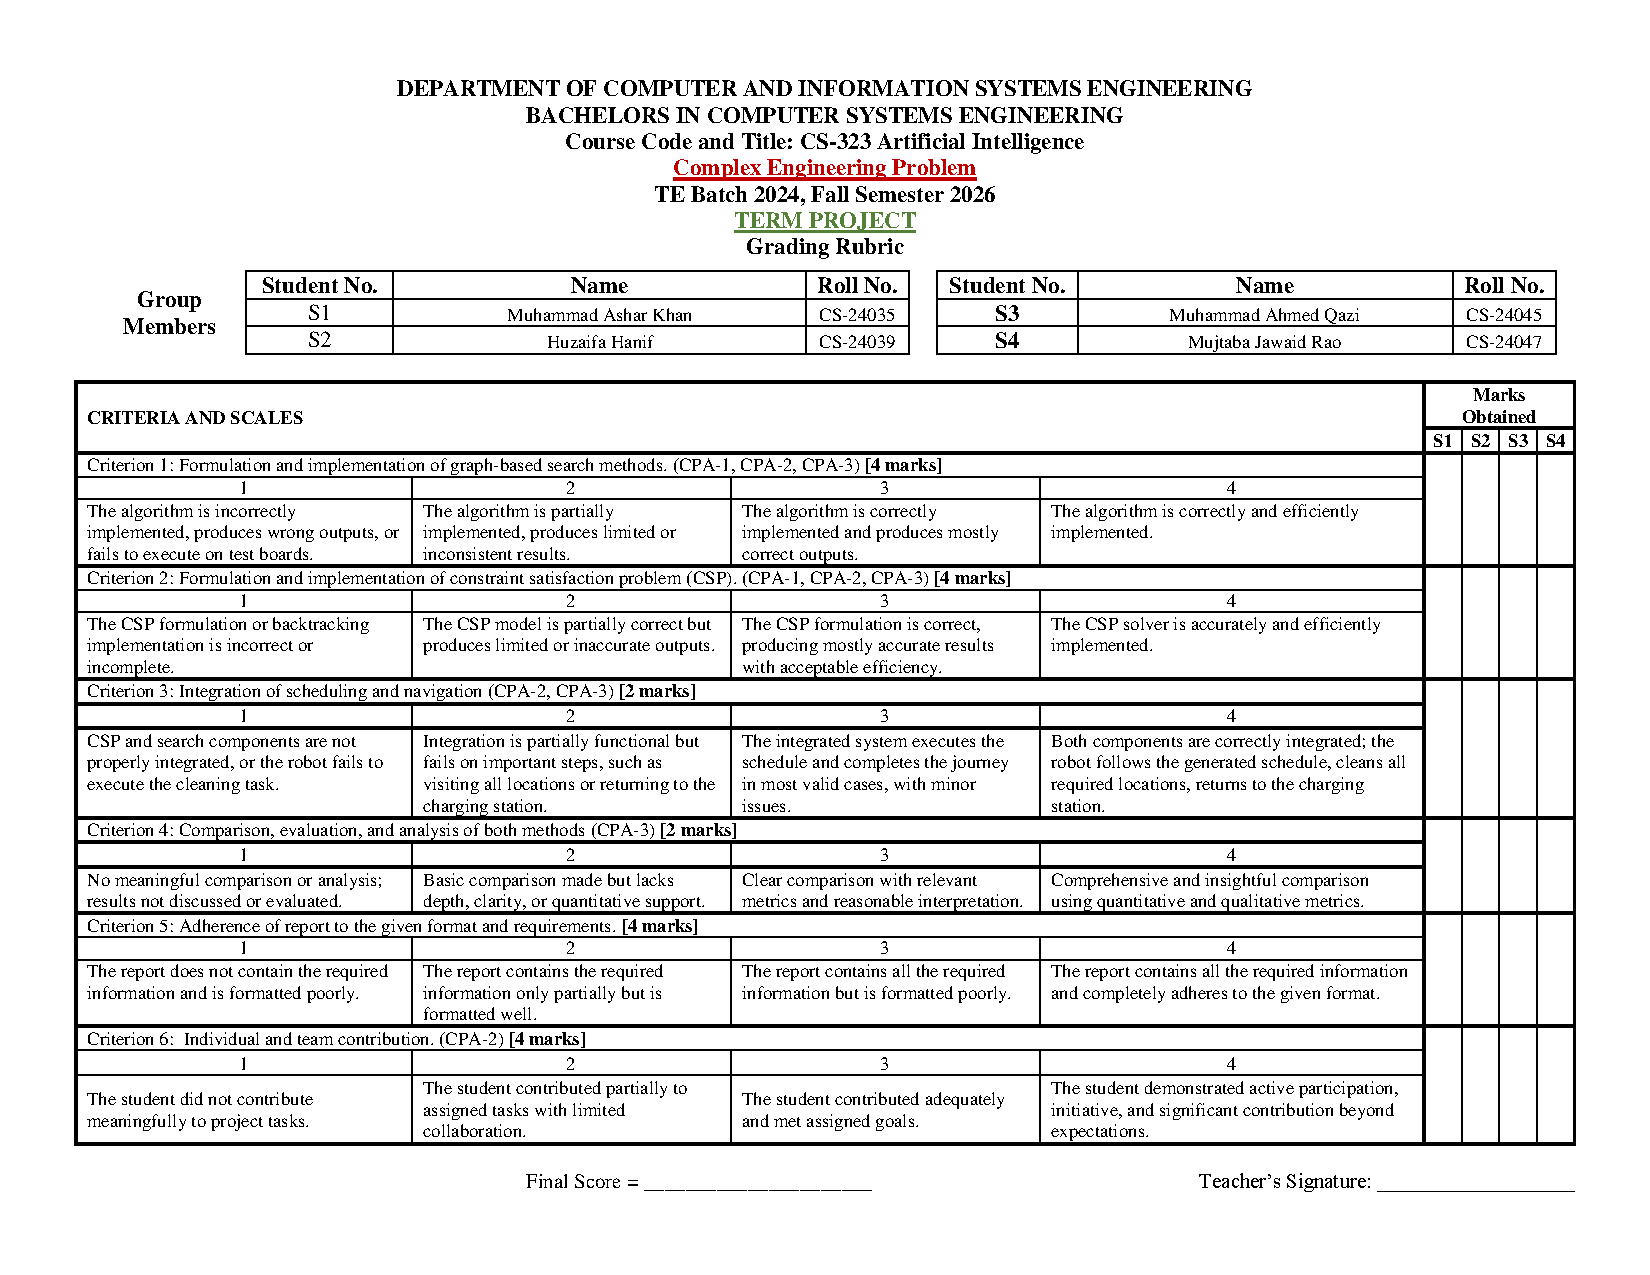
\includepdf[pages=1,fitpaper]{figures/rubric_filled.pdf}

% Page 1: table of contents (numbering starts here; the rubric is added separately).
\renewcommand{\contentsname}{Table of Contents}
% Main headings: solid rule to the page number; sub-items: dotted leader.
\titlecontents{section}[1.6em]{\addvspace{8pt}\bfseries}{\contentslabel{1.6em}}{\hspace*{-1.6em}}%
  {\hspace{4pt}\leaders\hrule height 0.4pt\hfill\hspace{4pt}\contentspage}
\titlecontents{subsection}[3.8em]{\addvspace{1pt}}{\contentslabel{2.2em}}{\hspace*{-2.2em}}%
  {\hspace{4pt}\titlerule*[0.5em]{.}\hspace{4pt}\contentspage}
% Same solid rule as the opening block, between the heading and the listing.
\makeatletter
\renewcommand\tableofcontents{\section*{\contentsname}\vspace{-4pt}%
  \noindent\rule{\linewidth}{0.6pt}\par\@starttoc{toc}}
\makeatother
\tableofcontents
\clearpage

% Opening block, on the same page as Section 1 (no title page, spec §8.2).
{\raggedright
\noindent\rule{\linewidth}{0.6pt}\par
\vspace{6pt}
{\fontsize{11}{13}\selectfont Complex Engineering Problem\par}
\vspace{4pt}
{\fontsize{14}{17}\selectfont\bfseries Intelligent Vacuum-Cleaning Robot: Graph Search and CSP Scheduling\par}
\vspace{10pt}
% Dotted grey divider between the title and the team list.
{\color{black!50}\noindent\leaders\hbox to 4pt{\hss\rule{1pt}{1pt}\hss}\hfill\null\par}
\vspace{10pt}
{\fontsize{11}{13}\selectfont
\textbf{Team Members:}\par
\vspace{-2pt}
\begin{itemize}[itemsep=5pt,topsep=2pt,parsep=0pt,leftmargin=1.4em]
  \item Muhammad Ashar Khan (CS-24035)
  \item Huzaifa Hanif (CS-24039)
  \item Muhammad Ahmed Qazi (CS-24045)
  \item Mujtaba Jawaid Rao (CS-24047)
\end{itemize}
\vspace{6pt}
\textbf{Notebook:} \code{CS24045.ipynb}\par
\vspace{4pt}
\textbf{To run the notebook, see \hyperref[app:run]{Appendix~A}.}\par
\vspace{10pt}
\itshape Design choices the specification leaves open are team decisions, recorded in our
decision log as \dec{01} to \dec{15}. They are cited by ID below and are not part of the
specification.\par}
\vspace{6pt}
\noindent\rule{\linewidth}{0.6pt}\par}

% !TEX root = ../main.tex
\section{Problem Definition and Representation}

A vacuum-cleaning robot works in a rectangular room divided into cells. Some cells are obstacles,
some are dirty, and one is the charging station. The robot must (1) choose a time slot for every
cleaning task so that all scheduling constraints hold, then (2) navigate from the charger to each
dirty cell in slot order and back to the charger, using graph search.

\textbf{Environment grid.} \code{Grid} is an immutable record with \code{rows}, \code{cols}, the set
of \code{obstacles}, the dirty cells \code{dirty} (label $\to$ cell, in file order, labels
D1\dots Dn) and the \code{charger} cell (\dec{06}). Coordinates are zero-based \code{(row, col)}
with \code{(0, 0)} at the top left. Dirty cells and the charger are passable; only obstacles and
out-of-bounds cells are blocked.

\textbf{Search problem (one navigation leg).}

\begin{center}
\begin{tabularx}{\linewidth}{@{}lX@{}}
\toprule
Element & Representation \\
\midrule
State & the robot's cell \code{(row, col)} \\
Initial state & the leg's start cell (charger or previous dirty cell) \\
Actions & UP $(-1,0)$, DOWN $(+1,0)$, LEFT $(0,-1)$, RIGHT $(0,+1)$, tried in that order (\dec{06}) \\
Transition model & \code{get\_successors(state, grid)}: apply the action; keep the result if it is inside the grid and not an obstacle \\
Goal test & \code{goal\_test(state, goal\_state)}: the robot is on the leg's target cell \\
Step cost & 1 per move; \code{path\_cost(path)} $=$ \code{len(path)} $-1$, and 0 for an empty path (\dec{04}) \\
\bottomrule
\end{tabularx}
\end{center}

\textbf{CSP (scheduling).} Variables are the task labels D1\dots Dn (all dirty cells, including
tasks with no constraint). The domain of each variable is the slots $\{1,\dots,T\}$, where $T$ comes
from line 1 of \code{Schedule.txt}; slots are integers and are shown as T1\dots T$T$ (\dec{06}).
There are three constraint types:
\begin{itemize}
  \item \emph{Precedence} $(D_i, D_j)$: $\mathrm{slot}(D_i) < \mathrm{slot}(D_j)$.
  \item \emph{Latest slot} $(D_i, T_k)$: $\mathrm{slot}(D_i) \le k$.
  \item \emph{Slot exclusivity} (implicit): no two tasks share a slot.
\end{itemize}

\textbf{Input formats.} \code{Environment.txt} has six lines: \code{rows,cols}; number of obstacles;
obstacle tuples; number of dirty cells; dirty-cell tuples; charger tuple. \code{Schedule.txt} has:
number of slots; number of precedence pairs; one \code{(Di,Dj)} per line; number of latest-slot
constraints; one \code{(Di,Tk)} per line. Both files are read at run time; nothing is hard-coded.
The parsers raise a single \code{InputError} naming the file, line and problem (\dec{07}). The rules
for whitespace, empty lists and value checks (duplicates, overlaps, out-of-bounds cells, unknown
labels) are \dec{08}--\dec{13}.

{\emergencystretch=3em Our own environment (\code{Environment.txt}) is a $10\times10$ room with 27 obstacles forming two
walls and a pocket, 5 dirty cells, and the charger at $(0,0)$. \code{Schedule.txt} has 6 slots, the
precedence chain D1$\to$D2$\to$D3$\to$D4, and the limits D4 $\le$ T4 and D2 $\le$ T3. D5 is
unconstrained, so it tests the ``every task gets a slot'' rule.\par}

% From Section 2 on, more space above each section heading (Section 1 keeps the default).
\titlespacing*{\section}{0pt}{24pt}{4pt}
% From Section 2 on, more space above each section heading (Section 1 keeps the default).
\titlespacing*{\section}{0pt}{24pt}{4pt}
% !TEX root = ../main.tex
\section{Graph-Based Search Algorithms}

We implemented Uniform-Cost Search (uninformed) and \astar{} (informed) (\dec{01}). Both are one
best-first \textbf{graph search} in \code{search(grid, start, goal, algorithm)}; they differ only in
the priority:
\begin{itemize}
  \item \textbf{UCS} expands the frontier node with the lowest path cost $g(n)$. With non-negative
    step costs, it is complete and optimal: when a node is removed from the frontier, its cheapest
    path is known.
  \item \textbf{\astar} expands the node with the lowest $f(n) = g(n) + h(n)$, where $h$ estimates
    the remaining cost. With a consistent $h$ it is complete and optimal, and it expands no node
    with $f > C^*$ (the optimal cost). This is why it usually expands fewer nodes than UCS.
\end{itemize}

Shared implementation details: a binary heap is the frontier. Ties are broken by insertion order,
so results are deterministic. A node is goal-tested when it is \emph{popped}, not when it is
generated, because testing on generation can return a non-optimal path. A \code{closed} set ensures
each cell is expanded at most once. A node counts as expanded when its successors are generated
(\dec{14}). \code{search} returns \code{(path, cost, nodes\_expanded)}, or
\code{(None, None, nodes\_expanded)} when no path exists; for start $=$ goal it returns
\code{([start], 0, 0)}. An unknown algorithm name raises \code{ValueError}.

\textbf{Heuristic choice.} For \astar{} we use Manhattan distance,
$h(n) = |row_n - row_{goal}| + |col_n - col_{goal}|$ (spec §5.5; \dec{02}). It is admissible:
each move is UP, DOWN, LEFT or RIGHT at cost 1, so one move reduces the Manhattan distance by at
most 1, and obstacles can only lengthen the real path. Hence $h(n)$ never exceeds the true remaining
cost. It is also consistent: for any move from $n$ to a neighbour $n'$, $h(n) \le 1 + h(n')$, and
$h(goal) = 0$. Because our \astar{} is a graph search with an explored set, consistency guarantees
that each cell is expanded first along a cheapest path. So \astar{} returns an optimal path with the
same cost as UCS, without reopening cells. Among admissible options it is the most informed:
Euclidean distance and $h = 0$ are never larger, so they would make \astar{} expand more nodes, and
$h = 0$ reduces \astar{} to UCS.

\begin{algorithm}[H]
\caption{Best-first graph search shared by UCS and \astar}
\begin{algorithmic}[1]
\Function{Search}{$grid, start, goal, algorithm$}
  \State $priority(n, g) \gets g + h(n, goal)$ \textbf{if} $algorithm = $ \astar{} \textbf{else} $g$ \Comment{UCS: $h \equiv 0$}
  \State $frontier \gets$ heap $\{(priority(start,0), start)\}$; \ $best\_g[start] \gets 0$
  \State $parent[start] \gets \textit{none}$; \ $closed \gets \emptyset$; \ $expanded \gets 0$
  \While{$frontier \neq \emptyset$}
    \State $n \gets$ pop lowest priority (FIFO among ties)
    \If{$n \in closed$} \textbf{continue} \Comment{stale duplicate entry}
    \EndIf
    \If{\Call{Goal-Test}{$n, goal$}}
      \State \Return $(\Call{Path}{parent, n},\ best\_g[n],\ expanded)$
    \EndIf
    \State $closed \gets closed \cup \{n\}$; \ $expanded \gets expanded + 1$
    \For{$(m, action, step) \in \Call{Get-Successors}{n, grid}$} \Comment{UP, DOWN, LEFT, RIGHT}
      \State $g \gets best\_g[n] + step$
      \If{$m \notin closed$ \textbf{and} $g < best\_g.\mathrm{get}(m, \infty)$}
        \State $best\_g[m] \gets g$; \ $parent[m] \gets n$
        \State push $(priority(m, g), m)$ onto $frontier$
      \EndIf
    \EndFor
  \EndWhile
  \State \Return $(\textit{None}, \textit{None}, expanded)$ \Comment{goal unreachable}
\EndFunction
\end{algorithmic}
\end{algorithm}

UCS is this procedure with $h \equiv 0$. \astar{} uses \code{heuristic(state, goal\_state)}.

% !TEX root = ../main.tex
\section{CSP Formulation and Implementation}

The formulation (variables, domains, three constraint types) is given in Section~1.
\code{Constraints} stores \code{variables} (file order), \code{num\_slots}, \code{precedence} pairs
and the \code{latest} map. Initial domains are $[1,\dots,T]$ for every variable. Before search
starts, \code{backtracking\_search} applies the unary latest-slot constraint to each domain (node
consistency). If any domain becomes empty, it returns \code{None} at once.

\textbf{The five required functions.}
\begin{itemize}
  \item \code{select\_unassigned\_variable} applies \textbf{MRV}: it picks the unassigned variable
    with the smallest current domain. Ties are broken by the \textbf{degree heuristic}: more
    \emph{distinct other unassigned variables} linked by a precedence constraint wins. Exclusivity
    links every pair equally, so it is not counted. Ties left after that go to file order
    D1\dots Dn (\dec{05}).
  \item \code{order\_domain\_values} applies \textbf{LCV} (optional in the spec, implemented). It
    sorts the variable's slots by how many values they would remove from the domains of other
    unassigned variables, fewest first. Python's stable sort keeps ascending slot order among ties.
  \item \code{is\_consistent} checks the proposed value against the latest-slot limit and against
    every \emph{already assigned} variable: no shared slot (exclusivity) and correct order for any
    precedence pair between them. Constraints with unassigned variables are left for forward
    checking.
  \item \code{forward\_check} copies the domains and, for each unassigned variable, removes every
    slot that would clash with the new assignment (same slot, or wrong side of a precedence pair).
    It returns the pruned copy, or \code{None} if some domain becomes empty (a dead end found early).
  \item \code{backtracking\_search} runs the recursive search below and returns a complete
    assignment, or \code{None} if no feasible schedule exists.
\end{itemize}

\textbf{Restoration.} \code{forward\_check} never changes the domains it is given; it works on a
copy. When a value fails, the recursion simply continues with the parent's unchanged domains. So
every value removed by forward checking is automatically ``restored'' on backtracking, and no undo
log is needed.

\begin{algorithm}[H]
\caption{Backtracking search with MRV, degree, LCV and forward checking}
\begin{algorithmic}[1]
\Function{Backtrack}{$assignment, domains, C$}
  \State $X \gets \Call{Select-Unassigned-Variable}{assignment, domains, C}$ \Comment{MRV, degree, file order}
  \If{$X = \textit{none}$} \Return copy of $assignment$ \Comment{all tasks scheduled}
  \EndIf
  \For{$v \in \Call{Order-Domain-Values}{X, assignment, domains, C}$} \Comment{LCV}
    \If{\textbf{not} \Call{Is-Consistent}{$X, v, assignment, C$}} \textbf{continue}
    \EndIf
    \State $assignment[X] \gets v$
    \State $pruned \gets \Call{Forward-Check}{X, v, assignment, domains, C}$ \Comment{works on a copy}
    \If{$pruned \neq \textit{None}$}
      \State $result \gets \Call{Backtrack}{assignment, pruned, C}$
      \If{$result \neq \textit{None}$} \Return $result$
      \EndIf
    \EndIf
    \State remove $X$ from $assignment$ \Comment{$domains$ unchanged $=$ restored}
  \EndFor
  \State \Return \textit{None}
\EndFunction
\Statex
\Function{Backtracking-Search}{$variables, domains, C$}
  \State $domains \gets$ each domain filtered by its latest-slot limit
  \If{some domain is empty} \Return \textit{None}
  \EndIf
  \State \Return \Call{Backtrack}{$\{\}, domains, C$}
\EndFunction
\end{algorithmic}
\end{algorithm}

On the sample files, the latest-slot filter leaves D2 and D3 with domain $\{1,2,3\}$. They tie on
MRV and on degree (one precedence neighbour each), so file order picks D2, and LCV places it in T1.
The resulting schedule is D2$\to$T1, D1$\to$T2, D3$\to$T3, D4$\to$T4. The notebook prints each
schedule together with a check of every constraint (Figures~\ref{fig:run1-schedule}, \ref{fig:run2-schedule} and~\ref{fig:run3-schedule}).

% !TEX root = ../main.tex
\section{System Integration}

{\emergencystretch=3em \code{execute\_\allowbreak schedule(grid, charging\_\allowbreak station, schedule, algorithm)} connects the two parts.
\code{plan\_\allowbreak and\_\allowbreak execute} first runs \code{backtracking\_search} on the parsed constraints. It then
converts the assignment into the \code{schedule}: the task labels sorted by slot, so empty slots are
skipped. Each label is mapped to its cell through \code{grid.dirty}. The integration only uses the
outputs of the CSP and of \code{search}; the visiting order and the paths are never hard-coded.\par}

\begin{algorithm}[!htbp]
\caption{Executing the CSP schedule with graph search}
\begin{algorithmic}[1]
\Function{Execute-Schedule}{$grid, charger, schedule, algorithm$}
  \State $stops \gets [\,grid.dirty[\ell] \text{ for } \ell \in schedule\,] + [charger]$
  \State $current \gets charger$; \ $complete\_path \gets [charger]$; \ $total \gets 0$
  \For{$target \in stops$}
    \State $(path, cost, nodes) \gets \Call{Search}{grid, current, target, algorithm}$
    \If{$path = \textit{None}$}
      \State \Return $(complete\_path, total, \textit{False})$ \Comment{failure, \dec{15}}
    \EndIf
    \State $complete\_path \gets complete\_path + path[1{:}]$ \Comment{drop repeated first cell}
    \State $total \gets total + cost$; \ $current \gets target$
    \If{$target \neq charger$} mark $target$ cleaned
    \EndIf
  \EndFor
  \State \Return $(complete\_path, total, \textit{True})$ \Comment{all cleaned, back at charger}
\EndFunction
\end{algorithmic}
\end{algorithm}

The grid is never changed; cleaned cells are tracked separately (\dec{06}). This way UCS and
\astar{} can run one after the other on the same \code{Grid}. For each algorithm, the notebook output
shows the schedule, the visit sequence, each leg's path with its cost and nodes expanded, the final
grid (\code{*} path, \code{dk} cleaned), the total moves and cost, and the final status.

\textbf{Failure handling (\dec{15}).} If a leg has no path, execution stops at that leg. It returns
the path walked so far, its cost, and \code{success = False}. The status line names the unreachable
leg, the tasks cleaned and not cleaned, and states that the robot did not return to the charger, so
the system never claims success. If the CSP finds no schedule, no search is run: the path is
\code{[charger]}, the cost is 0, and the run is reported as a failure. Input errors are caught and
reported as \code{InputError} messages, so the notebook does not crash.

% !TEX root = ../main.tex
\section{Results and Comparative Analysis}

All path costs and node counts below are deterministic, thanks to the FIFO tie-break. They come from
\code{tools/compare\_search.py} (the same code as notebook Section~4) and were re-run for this report:
costs and node counts were unchanged; only timings vary between machines.

\begin{table}[H]
\centering
\caption{Charger $\to$ each dirty cell on our \code{Environment.txt}.}
\begin{tabular}{@{}lcrrr@{}}
\toprule
Case & Path cost (UCS $=$ \astar) & Nodes UCS & Nodes \astar & \astar{} saving \\
\midrule
C$\to$D1 (3,4) & 11 & 41 & 23 & 44\,\% \\
C$\to$D2 (2,8) & 10 & 35 & 16 & 54\,\% \\
C$\to$D3 (9,9) & 18 & 72 & 59 & 18\,\% \\
C$\to$D4 (9,5) & 14 & 62 & 31 & 50\,\% \\
C$\to$D5 (9,0) & 13 & 54 & 19 & 65\,\% \\
\bottomrule
\end{tabular}
\end{table}

\begin{table}[H]
\centering
\caption{Scaling on open $n\times n$ grids: nodes expanded (UCS and \astar{} path costs equal).}
\begin{tabular}{@{}rcc@{}}
\toprule
$n$ & Corner $(0,0)\to(n{-}1,n{-}1)$: UCS / \astar & Midline left$\to$right: UCS / \astar \\
\midrule
5 & 24 / 24 & 18 / 4 \\
10 & 99 / 99 & 74 / 9 \\
20 & 399 / 399 & 299 / 19 \\
40 & 1599 / 1599 & 1199 / 39 \\
80 & 6399 / 6399 & 4799 / 79 \\
\bottomrule
\end{tabular}
\end{table}

\begin{figure}[H]
\centering
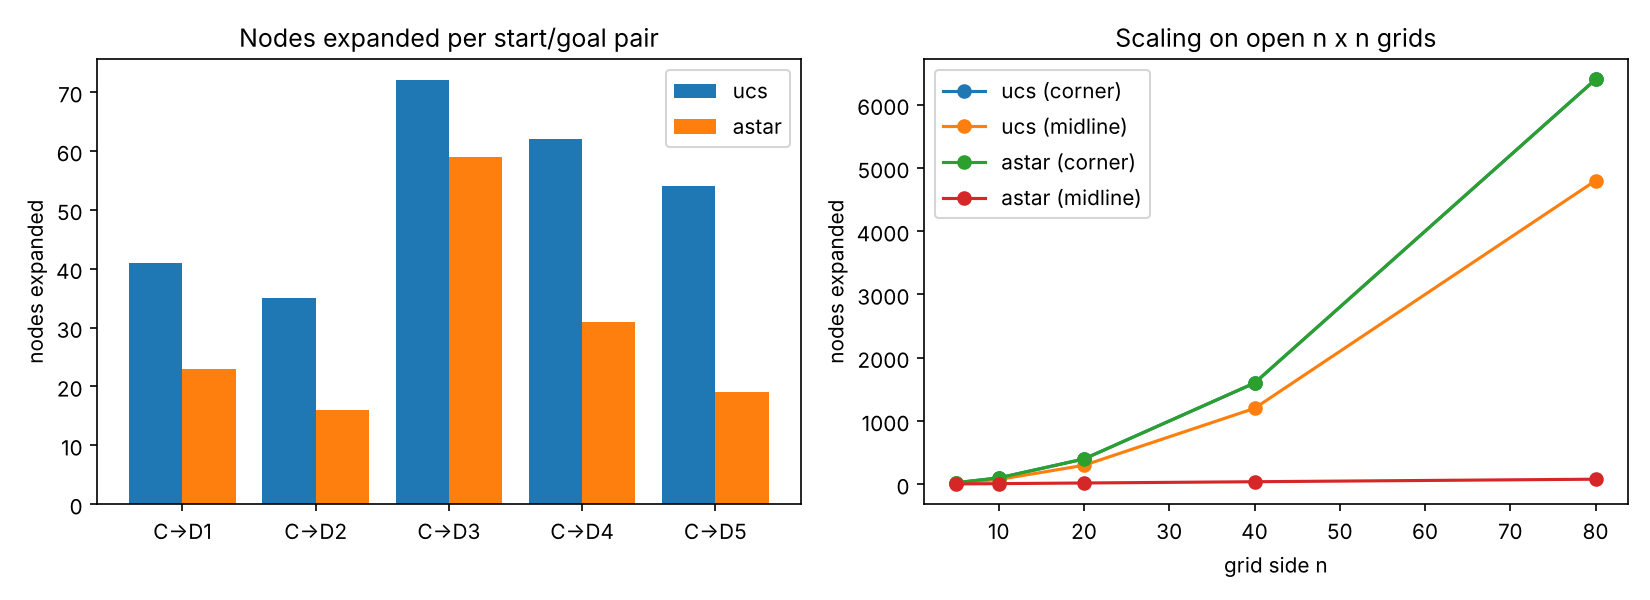
\includegraphics[width=\linewidth]{search_comparison.png}
\caption{Nodes expanded per start/goal pair on our environment (left) and scaling on open grids (right).}
\label{fig:compare}
\end{figure}

\begin{table}[H]
\centering
\caption{Full integrated runs (CSP schedule $+$ navigation, all legs including the return).}
\begin{tabular}{@{}llcrrl@{}}
\toprule
Files & Schedule & Moves $=$ cost & Nodes UCS & Nodes \astar & Status \\
\midrule
Own & D1, D2, D3, D4, D5 & 64 & 253 & 112 & success (both) \\
Sample & D2, D1, D3, D4 & 34 & 139 & 52 & success (both) \\
Error & D1, D2, D3, D4, D5 & 46 (stopped) & 259 & 156 & failure: D5 unreachable \\
\bottomrule
\end{tabular}
\end{table}

\textbf{Discussion.}
\begin{itemize}
  \item \emph{Path cost.} UCS and \astar{} found paths of equal cost in every run, as expected: both
    are optimal (Manhattan distance is admissible and consistent). The \emph{paths} can still differ
    when several optimal paths exist. On our grid, the leg C$\to$D1 goes via (4,0),(5,0) under UCS
    and via (3,1),(4,1) under \astar; both have cost 11 (Figures~\ref{fig:run1-ucs} and~\ref{fig:run1-astar}).
  \item \emph{Nodes expanded.} On our environment, \astar{} expanded 18--65\,\% fewer nodes per pair,
    and 56\,\% fewer over the whole integrated route (112 vs 253). The smallest gain is C$\to$D3: the
    walls force a long detour, so Manhattan distance underestimates more and many cells share the
    lowest $f$.
  \item \emph{Geometry decides the benefit.} On an open grid from corner to corner, every cell in the
    bounding box has the same $f = 2(n-1)$. The heuristic then cannot rule anything out, and \astar{}
    ties UCS at $n^2-1$ nodes. Along the midline only one shortest path exists, so \astar{} expands
    exactly $n-1$ nodes (linear), while UCS grows a ``diamond'' of equal $g$ around the start (about
    $0.75\,n^2$). At $80\times80$ this is 79 versus 4799.
  \item \emph{Time and memory.} Per node, \astar{} does slightly more work (one heuristic call per
    push), which is visible where both expand the same nodes. Whenever \astar{} expands fewer nodes,
    it also wins on time and frontier size.
  \item \emph{Unreachable goal.} Both algorithms expanded all 69 cells reachable from D4 in the error
    grid before reporting ``no path''. With no path to find, the heuristic gives no saving.
\end{itemize}

% !TEX root = ../main.tex
\section{Testing and Validation}

We ran the notebook end to end on three file pairs (spec §8.2). For each run, the configuration is
the content of the two input files, shown as a screenshot of the files as read from disk. The output
is shown in three screenshots of the notebook cell: the parsed grid with the CSP schedule and its
constraint check, then the integration output for UCS, then for \astar.

\subsection{Test run 1: our files (\code{Environment.txt}, \code{Schedule.txt})}
The schedule is D1\dots D5 in T1\dots T5, with T6 empty, and all constraints are satisfied. Both
algorithms clean all five cells and return to the charger: 64 moves, cost 64, status SUCCESS.

\figcenterbegin
\begin{figure}[H]
\centering
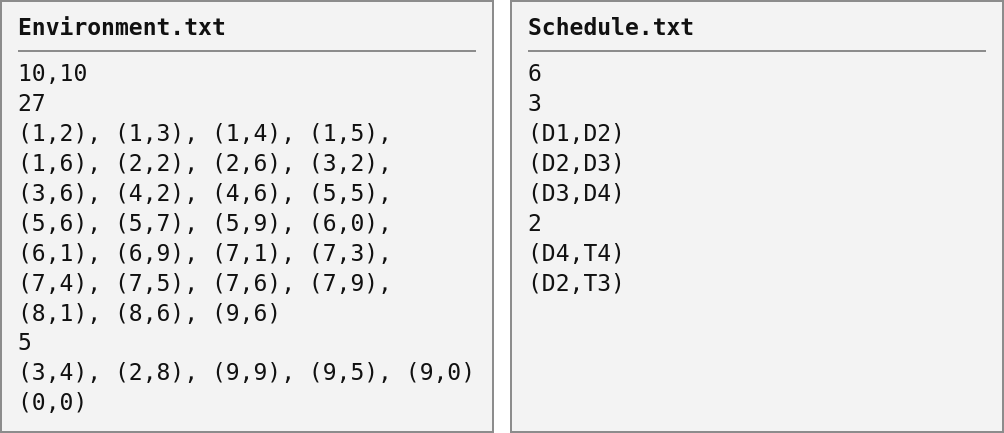
\includegraphics[width=0.8\linewidth]{run1_config.png}
\caption{Test run 1 (own files): configuration, the environment and schedule input files.}
\label{fig:run1-config}
\end{figure}
\figcenterend

\figcenterbegin
\begin{figure}[H]
\centering
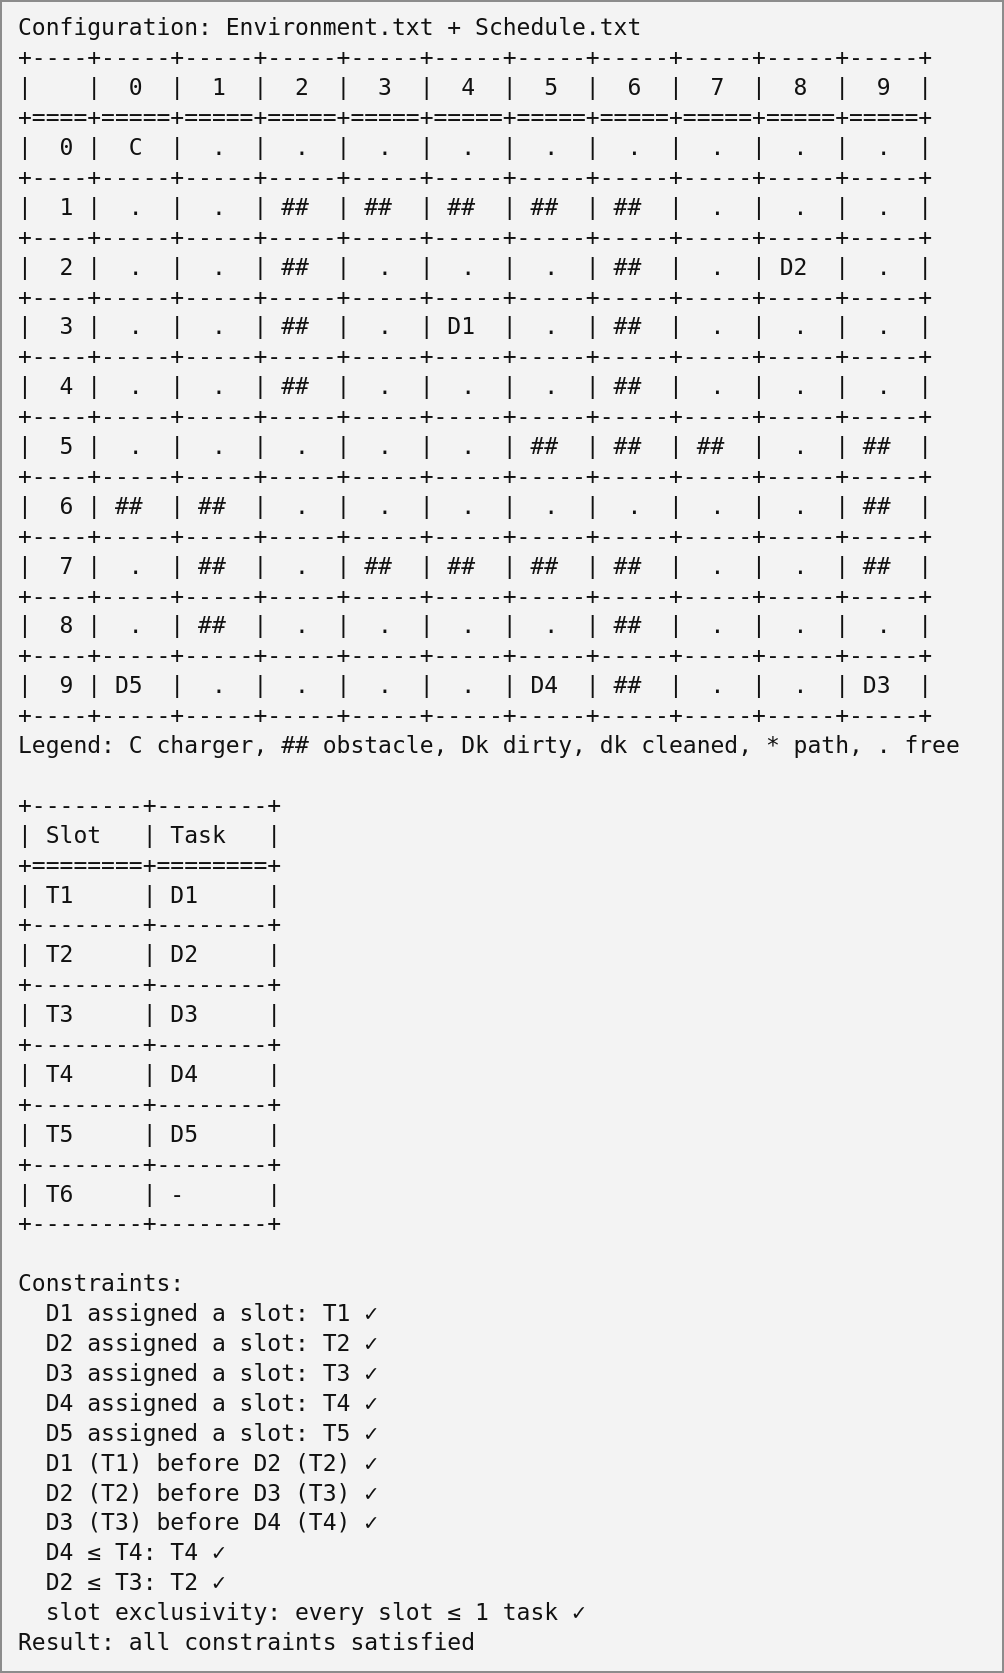
\includegraphics[width=0.8\linewidth]{run1_schedule.png}
\caption{Test run 1 (own files): parsed grid, CSP schedule and constraint check.}
\label{fig:run1-schedule}
\end{figure}
\figcenterend

\figcenterbegin
\begin{figure}[H]
\centering
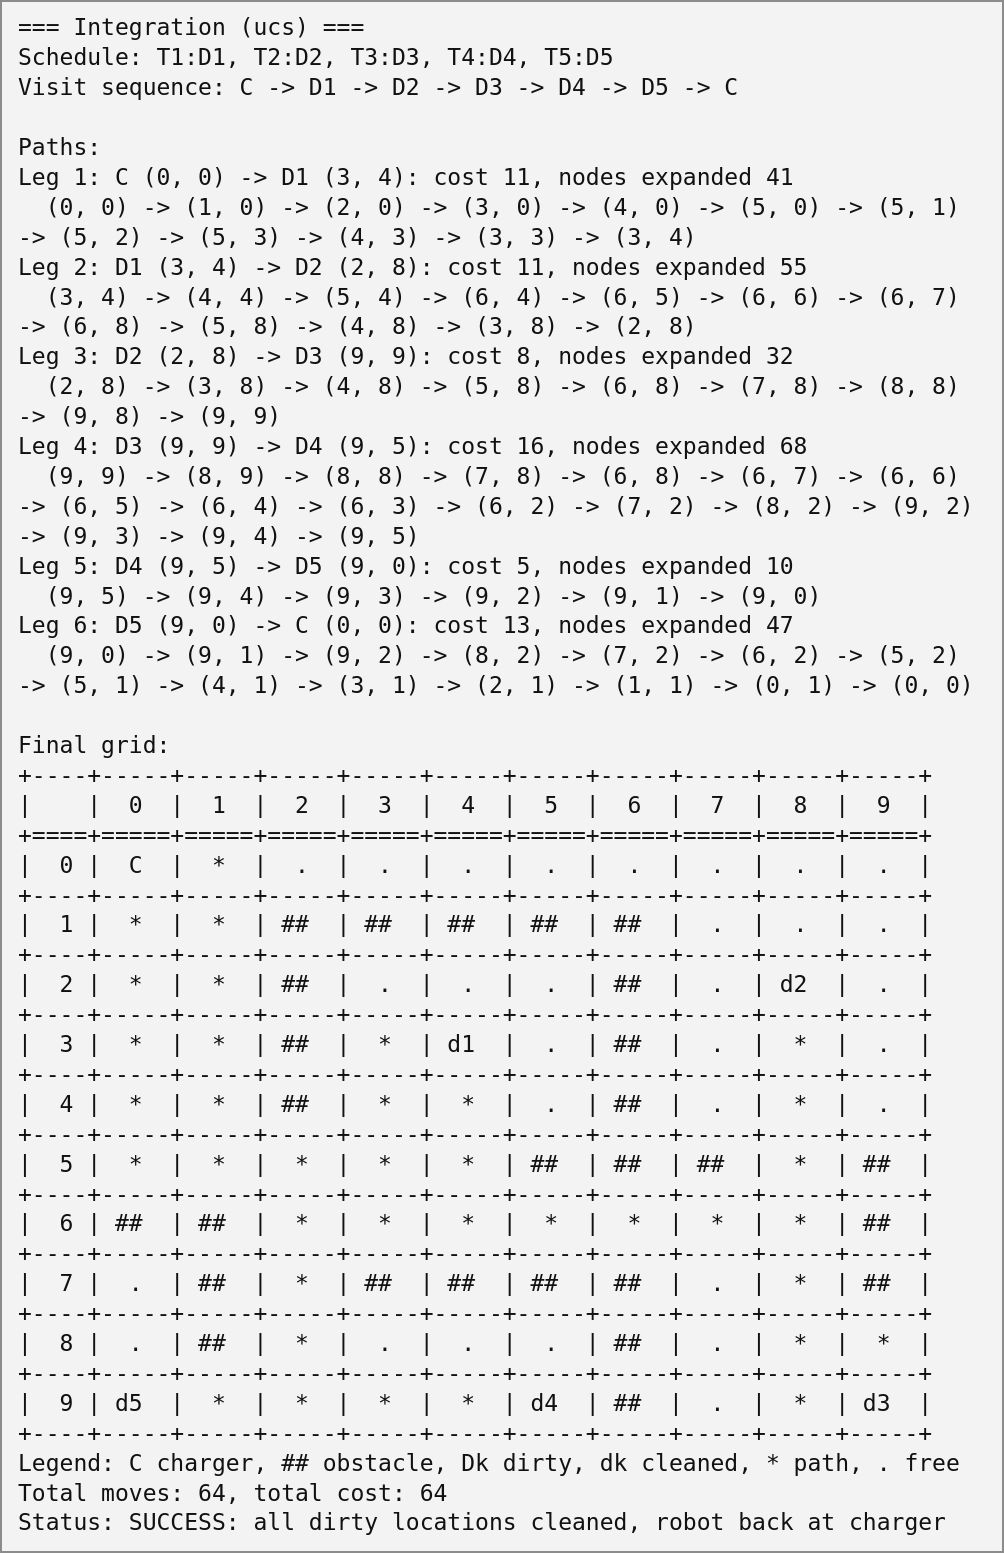
\includegraphics[width=0.8\linewidth]{run1_ucs.png}
\caption{Test run 1 (own files): integration output with UCS.}
\label{fig:run1-ucs}
\end{figure}
\figcenterend

\figcenterbegin
\begin{figure}[H]
\centering
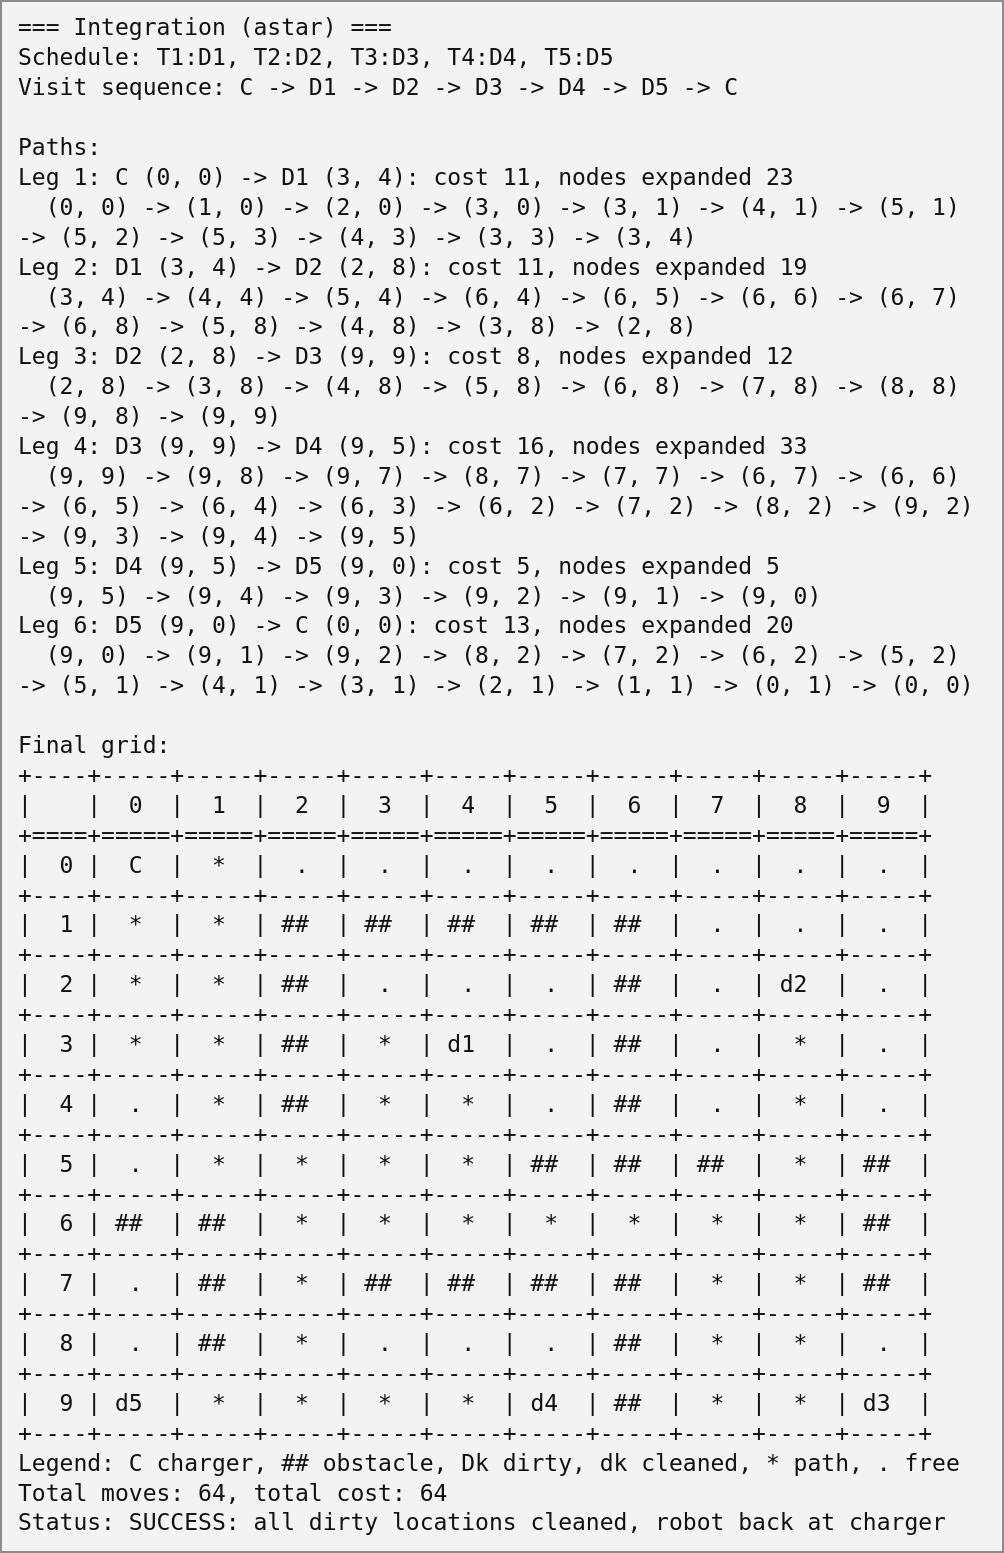
\includegraphics[width=0.8\linewidth]{run1_astar.png}
\caption{Test run 1 (own files): integration output with \astar.}
\label{fig:run1-astar}
\end{figure}
\figcenterend


\newpage
\subsection{Test run 2: provided sample (\code{Environment\_Sample.txt}, \code{Schedule\_Sample.txt})}
The schedule is T1:D2, T2:D1, T3:D3, T4:D4, and all constraints are satisfied. Both algorithms
finish with 34 moves, cost 34, status SUCCESS.

\figcenterbegin
\begin{figure}[H]
\centering
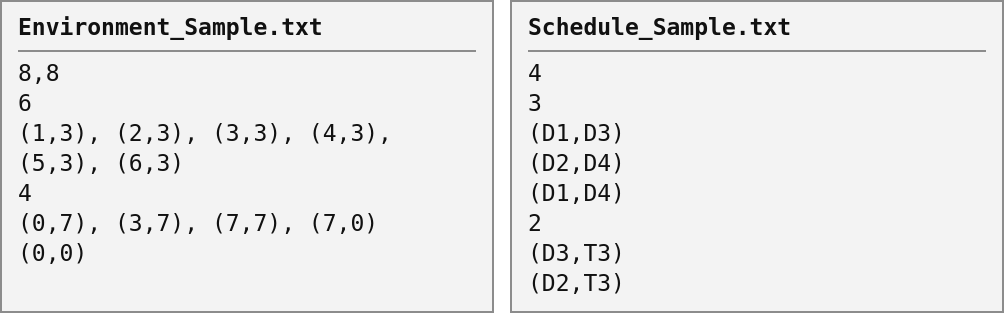
\includegraphics[width=0.8\linewidth]{run2_config.png}
\caption{Test run 2 (sample files): configuration, the environment and schedule input files.}
\label{fig:run2-config}
\end{figure}
\figcenterend

\figcenterbegin
\begin{figure}[H]
\centering
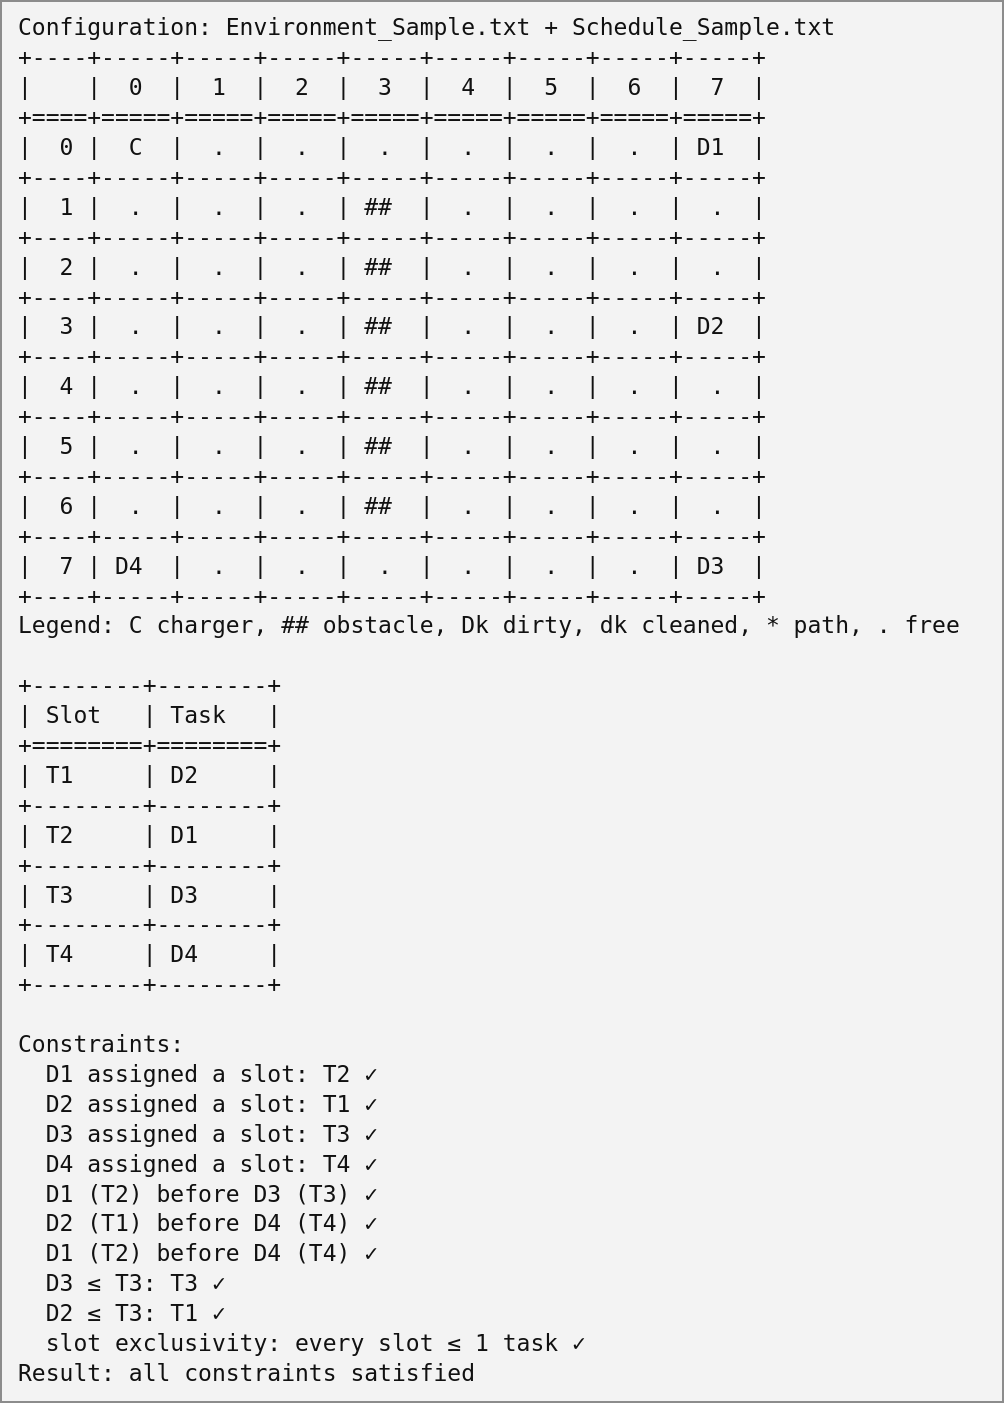
\includegraphics[width=0.8\linewidth]{run2_schedule.png}
\caption{Test run 2 (sample files): parsed grid, CSP schedule and constraint check.}
\label{fig:run2-schedule}
\end{figure}
\figcenterend

\figcenterbegin
\begin{figure}[H]
\centering
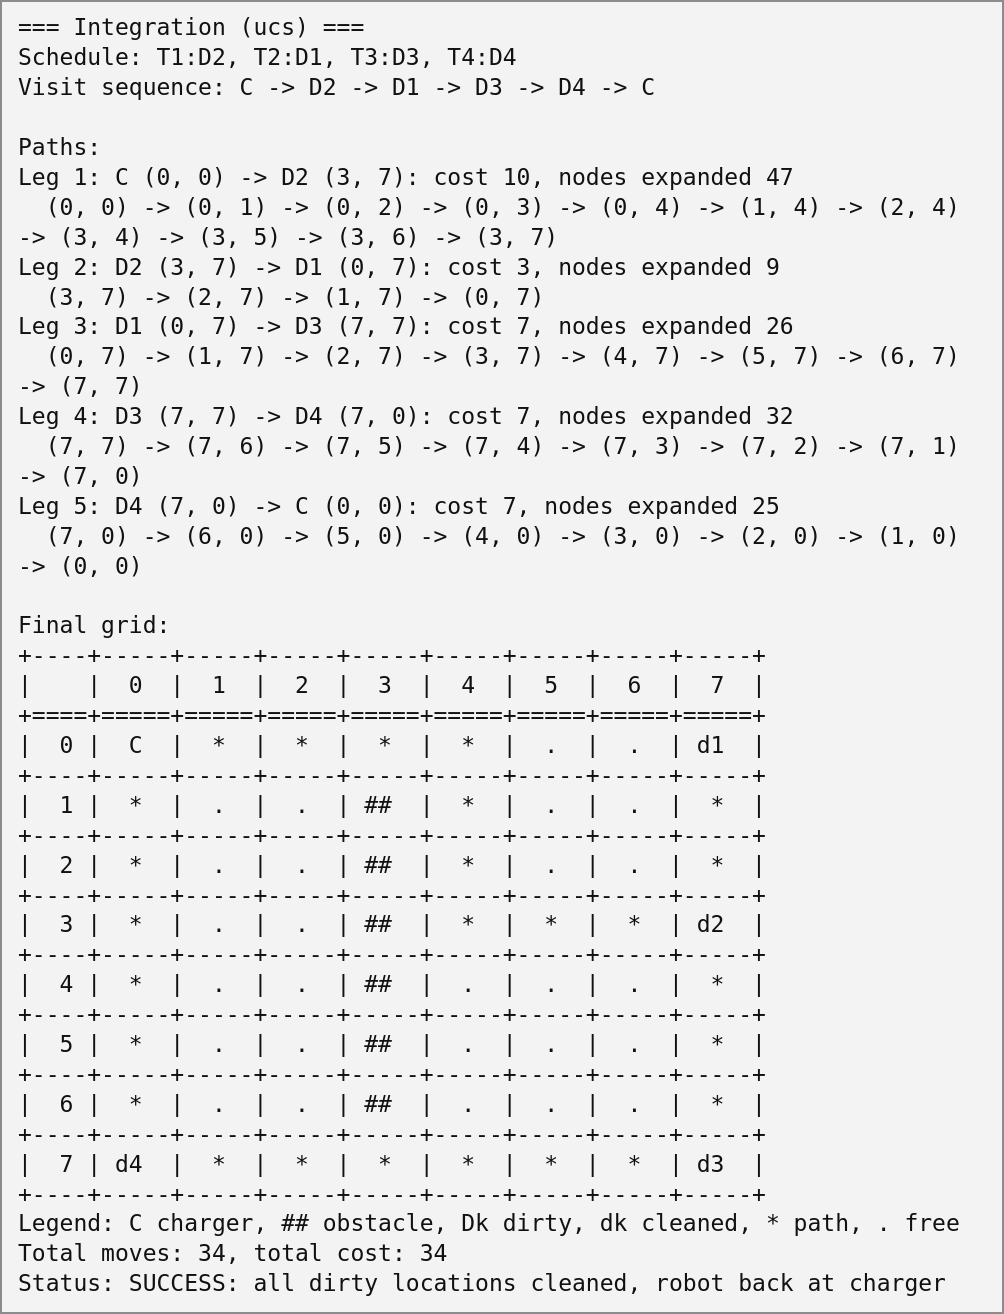
\includegraphics[width=0.8\linewidth]{run2_ucs.png}
\caption{Test run 2 (sample files): integration output with UCS.}
\label{fig:run2-ucs}
\end{figure}
\figcenterend

\figcenterbegin
\begin{figure}[H]
\centering
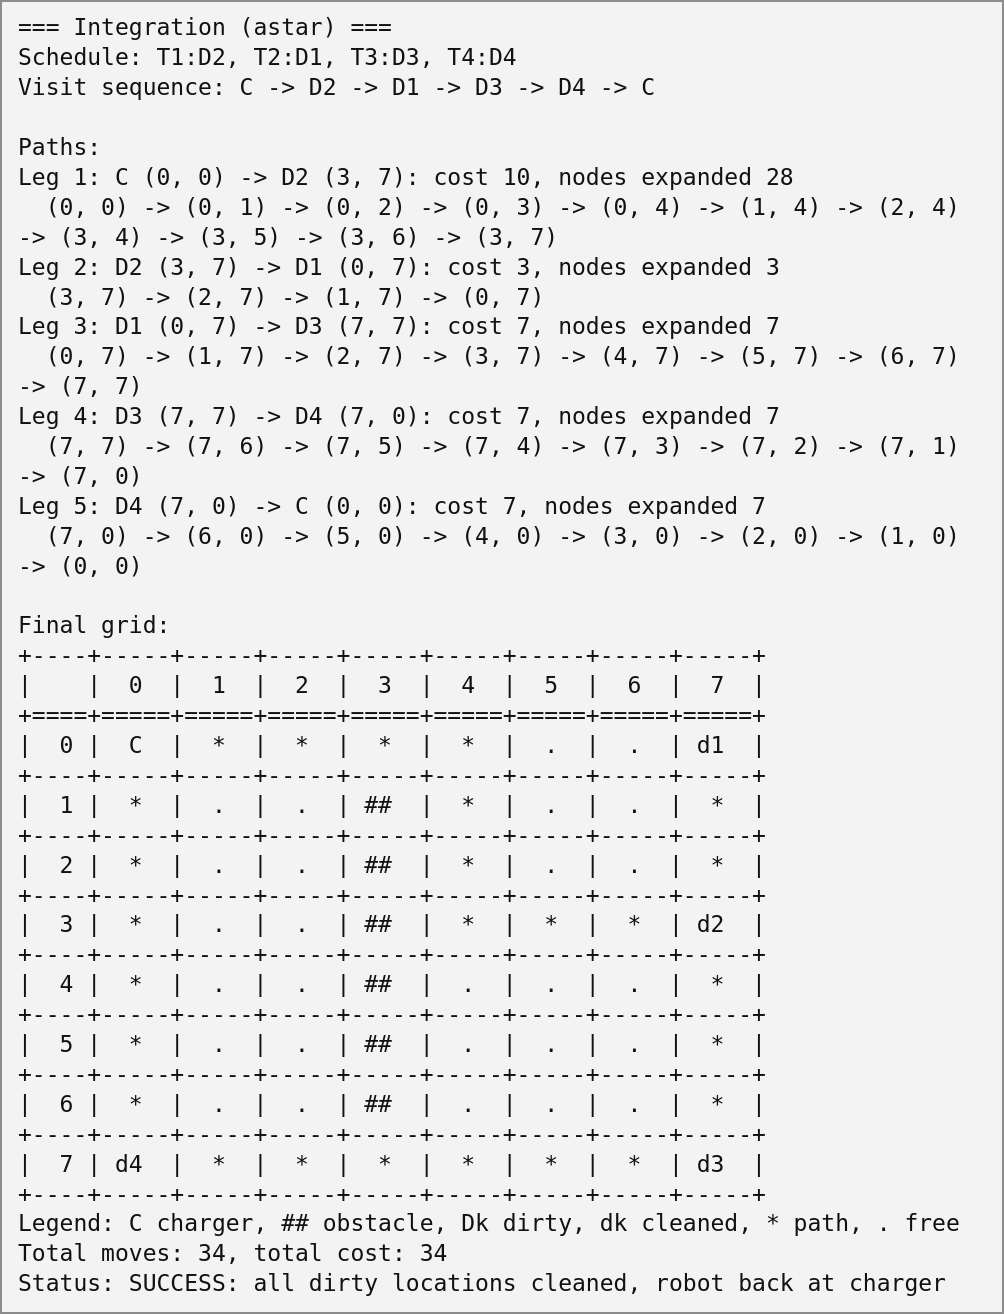
\includegraphics[width=0.8\linewidth]{run2_astar.png}
\caption{Test run 2 (sample files): integration output with \astar.}
\label{fig:run2-astar}
\end{figure}
\figcenterend

\newpage
\subsection{Test run 3: failure case (\code{Environment\_Error.txt}, \code{Schedule\_Error.txt})}
This is our environment with two extra obstacles at (8,0) and (9,1), which wall in D5 at (9,0).
The schedule is unchanged and still feasible, so the CSP succeeds. The leg D4$\to$D5 then returns no
path (69 nodes expanded). The system stops there and prints
\code{FAILURE: no path from D4 (9, 5) to D5 (9, 0)}, lists D1--D4 as cleaned and D5 as not cleaned,
and states that the robot did not return to the charger. The final grid shows D5 still dirty
(Figures~\ref{fig:run3-ucs} and~\ref{fig:run3-astar}).

\figcenterbegin
\begin{figure}[H]
\centering
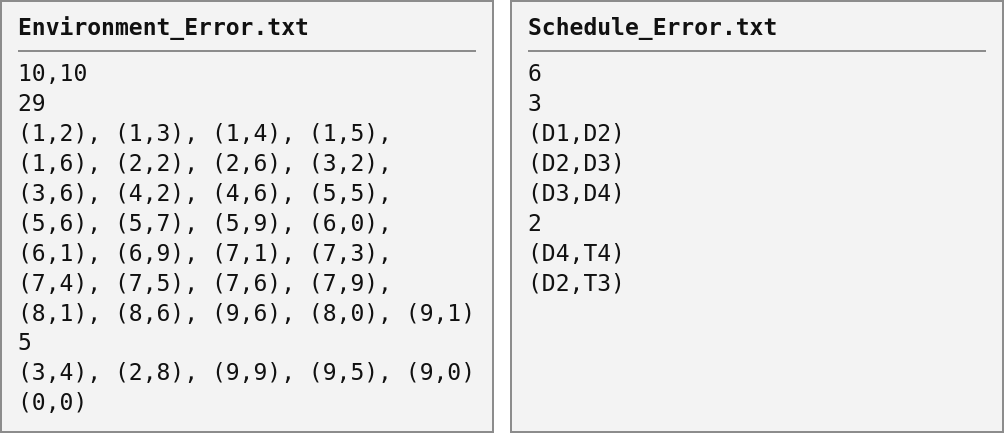
\includegraphics[width=0.8\linewidth]{run3_config.png}
\caption{Test run 3 (error files): configuration, the environment and schedule input files.}
\label{fig:run3-config}
\end{figure}
\figcenterend

\figcenterbegin
\begin{figure}[H]
\centering
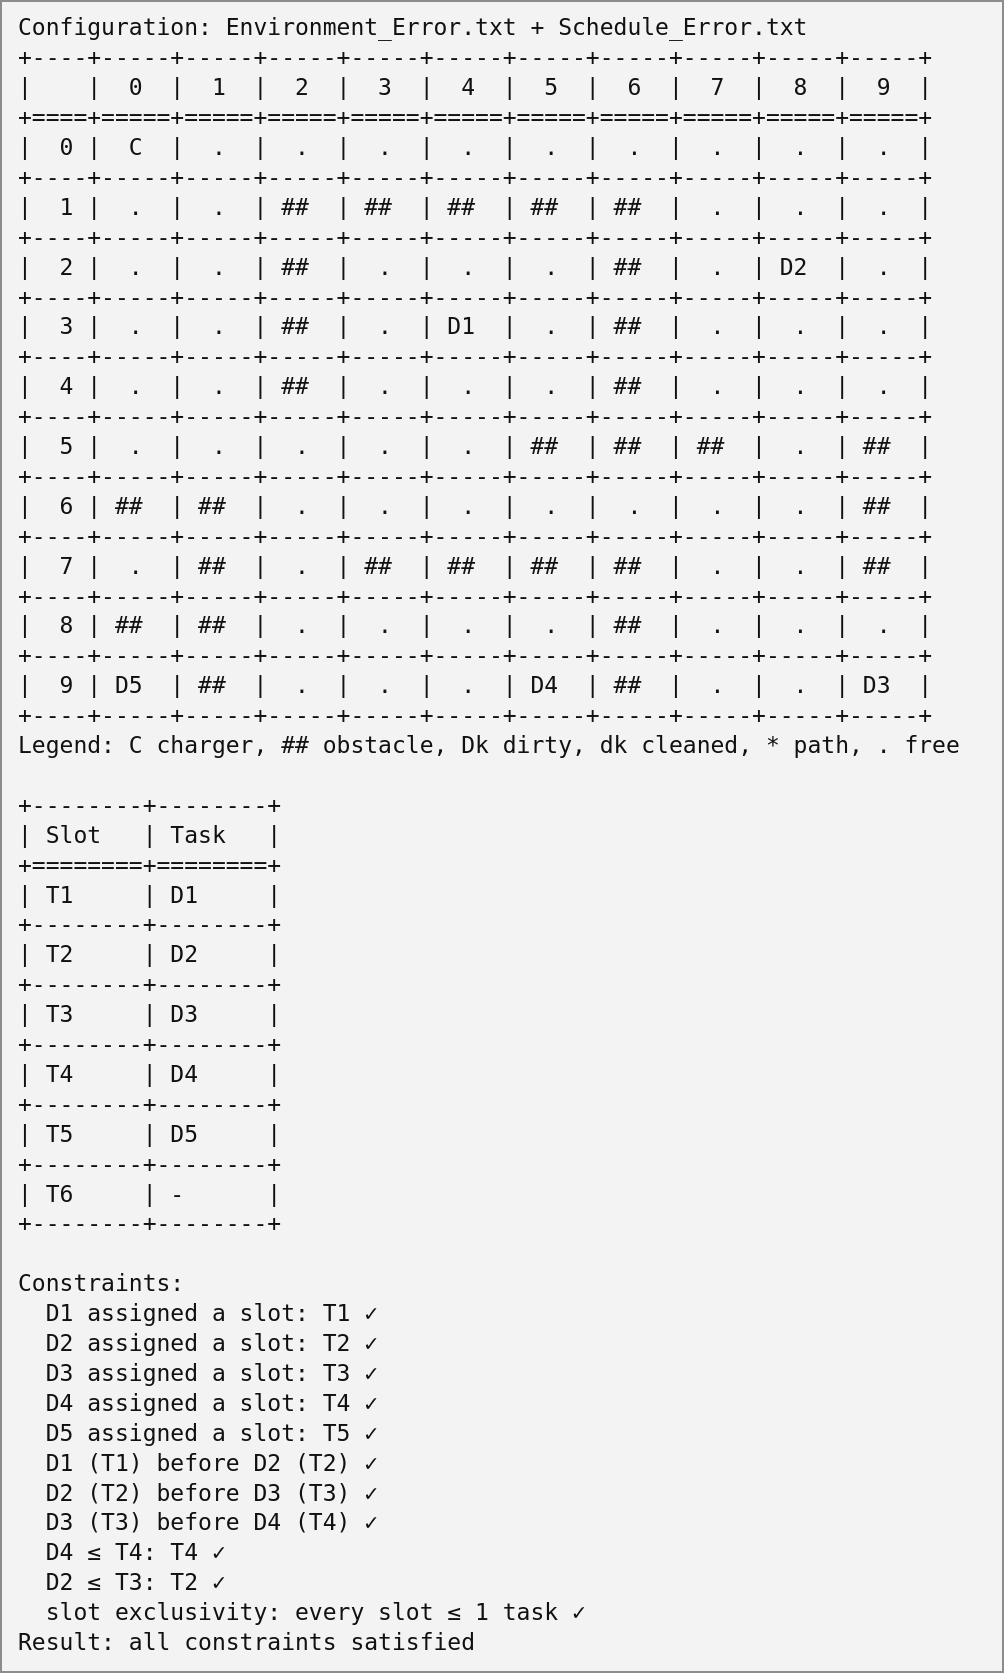
\includegraphics[width=0.8\linewidth]{run3_schedule.png}
\caption{Test run 3 (error files): parsed grid, CSP schedule and constraint check.}
\label{fig:run3-schedule}
\end{figure}
\figcenterend

\figcenterbegin
\begin{figure}[H]
\centering
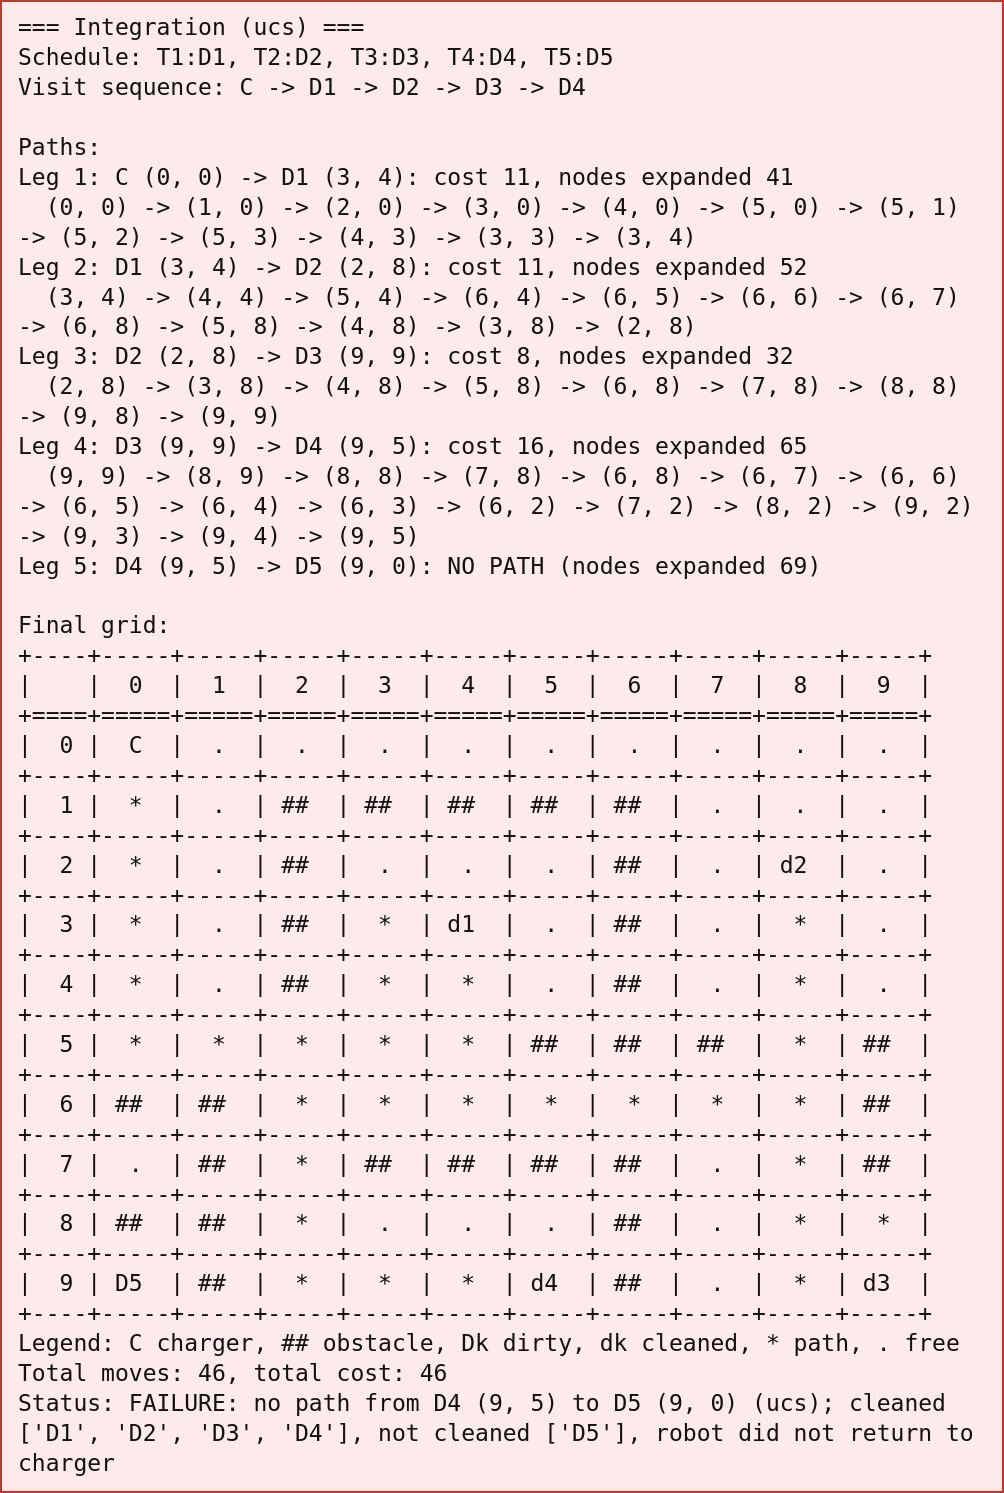
\includegraphics[width=0.8\linewidth]{run3_ucs.png}
\caption{Test run 3 (error files): integration output with UCS.}
\label{fig:run3-ucs}
\end{figure}
\figcenterend

\figcenterbegin
\begin{figure}[H]
\centering
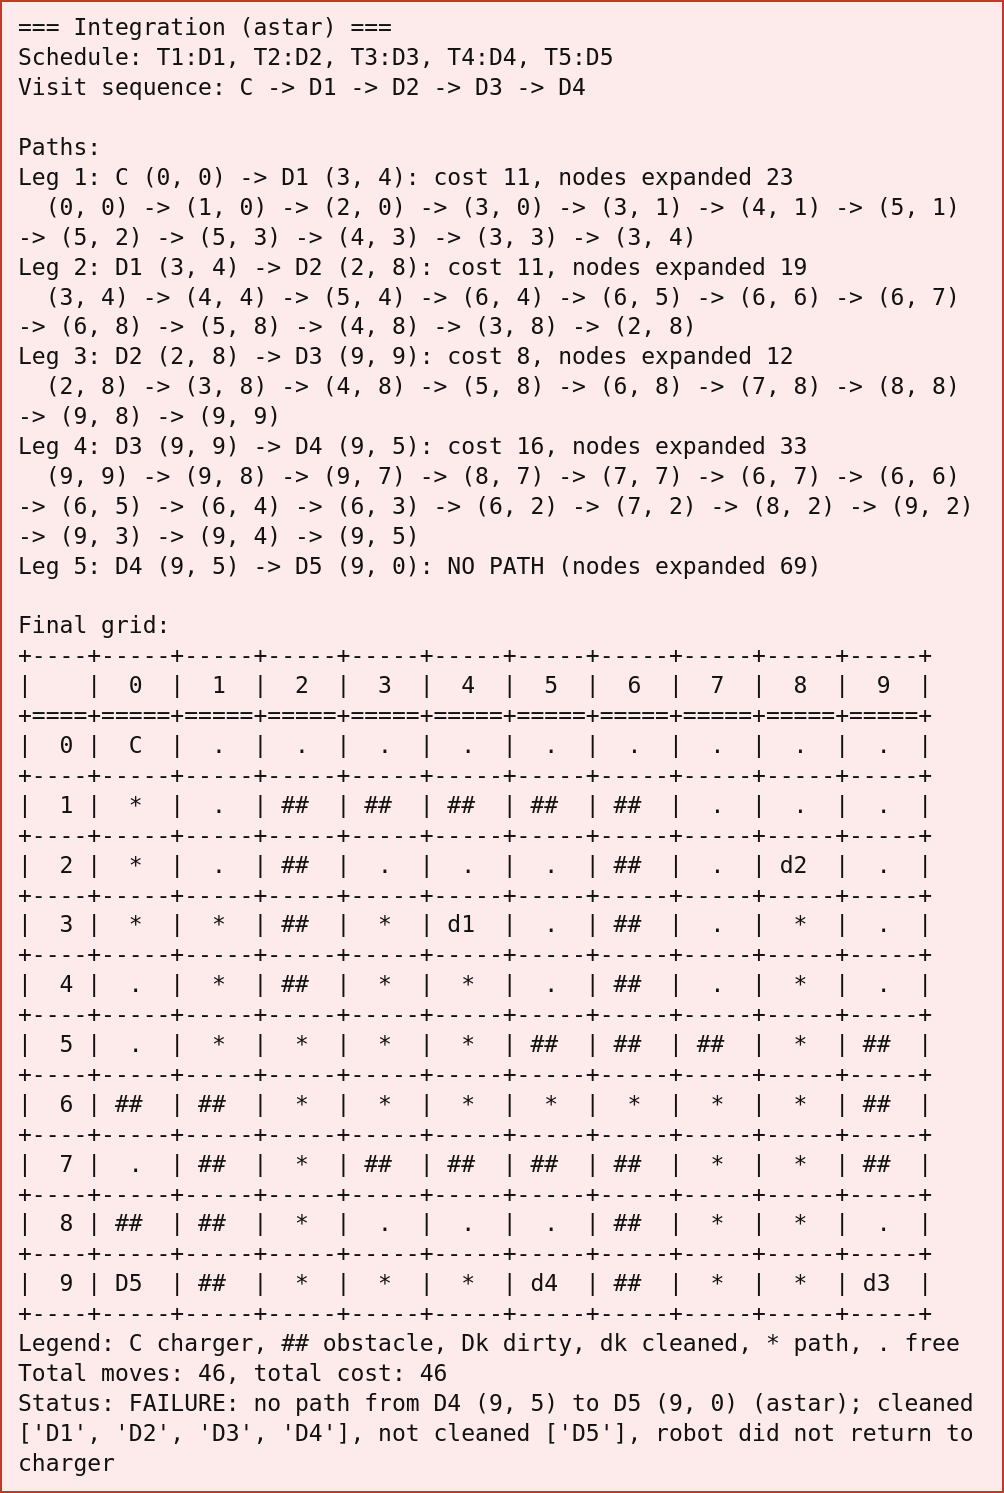
\includegraphics[width=0.8\linewidth]{run3_astar.png}
\caption{Test run 3 (error files): integration output with \astar.}
\label{fig:run3-astar}
\end{figure}
\figcenterend


\newpage
\subsection{Automated tests}
{\emergencystretch=3em In addition to the three runs, \code{pytest} runs 94 tests (all passing).
They cover the parsers (valid files, the sample files, and each invalid-input rule), successors,
path cost, the heuristic and both search algorithms (including start $=$ goal and no path; costs on
many start/goal pairs of our grid are checked against a breadth-first-search distance), the CSP
functions (checked against a brute-force solver that tries every assignment), integration (success,
an unreachable leg, an infeasible schedule) and the display. A seeded generator
(\code{tools/gen\_env.py}) produces random reachable/unreachable environments and
feasible/infeasible schedules; property-based tests (Hypothesis) check that the generated files
parse and have the requested properties. Continuous integration runs lint, tests, robustness,
interface checks, and a full execution of the notebook on every pull request.\par}

% !TEX root = ../main.tex
\section{Discussion and Improvements}

\textbf{Correctness, completeness and optimality.} The grid is finite and every graph search keeps a
closed set, so UCS and \astar{} are complete: each returns a path if one exists and reports failure
otherwise (test run 3). With unit step costs, UCS is optimal. \astar{} with consistent Manhattan
distance is optimal and never needs to reopen a cell. Every run in Section~5 confirmed equal costs.
The backtracking CSP solver is complete: forward checking only removes values that cannot appear in
any solution extending the current assignment. So if a schedule exists it is found, and otherwise
\code{None} is returned. The brute-force comparison in the test suite confirms this on small
instances.

\textbf{Performance.} \astar{} never did worse than UCS in nodes expanded. Its saving ranges from
none on open, symmetric layouts to linear-versus-quadratic on corridor-like routes. The CSP
instances are tiny; with MRV $+$ degree, LCV and forward checking, the sample and our schedule are
solved without backtracking.

\textbf{Limitations.}
\begin{itemize}
  \item The visiting order is fixed by the slot order. The robot's total route is therefore optimal
    \emph{for that schedule}, not the shortest tour over all feasible schedules.
  \item One unreachable task stops the whole run (\dec{15}). Later reachable tasks are not
    attempted, and the robot is not returned to the charger.
  \item Movement is 4-directional with unit cost. There is no battery, time-per-move, or
    dynamic-obstacle model.
  \item Paths are recomputed for every leg and every algorithm. There is no caching of distances.
\end{itemize}

\textbf{Improvements.}
\begin{itemize}
  \item Choose among feasible schedules by route length: compute pairwise distances between all
    stops with search, then minimise the tour cost subject to the CSP constraints (for example,
    branch and bound over the CSP solutions).
  \item On an unreachable task, skip it, continue with the remaining reachable tasks, and return to
    the charger, then report partial success.
  \item Use stronger propagation (AC-3) or detect precedence cycles before search, for larger
    schedules.
  \item Tie-break \astar{} on larger $g$ among equal $f$, which reduces expansions on open grids
    where many cells tie (the corner case in Table~2).
\end{itemize}

% !TEX root = ../main.tex
\section{References}
\begin{enumerate}[label={[\arabic*]}]
  \item S.~Russell and P.~Norvig, \emph{Artificial Intelligence: A Modern Approach}, 4th ed.
    Pearson, 2020. Ch.~3 (uninformed and informed search, \astar, admissibility and consistency)
    and Ch.~6 (CSPs, backtracking, MRV, degree, LCV, forward checking).
  \item P.~E.~Hart, N.~J.~Nilsson and B.~Raphael, ``A Formal Basis for the Heuristic Determination
    of Minimum Cost Paths,'' \emph{IEEE Trans.\ Systems Science and Cybernetics}, vol.~4, no.~2,
    pp.~100--107, 1968.
  \item CS-323 Artificial Intelligence, \emph{Complex Engineering Problem: Problem Description and
    Instructions} and \emph{Grading Rubric}, Fall 2026.
  \item Python Software Foundation, \code{heapq} --- Heap queue algorithm, Python~3 documentation.
    \url{https://docs.python.org/3/library/heapq.html}
  \item Hypothesis (property-based testing for Python), \url{https://hypothesis.readthedocs.io}
\end{enumerate}

% !TEX root = ../main.tex
\section{Generative AI Use Declaration}

\textbf{Generative AI tools were used in this project.} The tools were Claude Code (Anthropic, model
Claude Opus 5.5), used by Qazi, Mujtaba and Huzaifa, and ChatGPT (OpenAI, GPT-6), used by Ashar.
Every use was recorded in our AI use log (date, member, tool, purpose, issue).

\textbf{Purposes.}
\begin{itemize}
  \item \emph{Project setup and planning:} repository layout, continuous integration, templates, and
    the requirement list derived from the specification. Recording design decisions after the team
    chose among the options (\dec{01}--\dec{15}).
  \item \emph{Code authoring} (allowed by a team decision on 18 Nov): the environment and schedule
    parsers, the search functions (UCS/\astar, heuristic), the comparison tooling, the CSP solver,
    integration, display, the notebook builder, and parts of the tests and the random file
    generator. The members who own each part reviewed it, ran the tests, and are prepared to explain
    it at the viva.
  \item \emph{Debugging and validation:} a fix to the local CI script, checks of our own and error
    input files, and test reviews.
  \item \emph{Report writing:} the heuristic justification paragraph and the search-comparison
    analysis draft were AI-written. \textbf{This report draft was also written with Claude Code}
    from our code, decision log and measured results, and converted to LaTeX with it. The notebook's
    markdown cells and the test-run screenshots were also AI-assisted. All numbers in this report
    come from running the submitted code.
\end{itemize}

\textbf{Responsibility.} The group reviewed and understood the implementation, the results and this
report, checked them against the specification, and takes full responsibility for the submitted
work.


% Appendix after the Generative AI Use Declaration (Section 9).
\appendix
\newpage
% !TEX root = ../main.tex
\section[\texorpdfstring{\protect\fbox{\strut Quick Guide: Running the Notebook}\protect\hspace{6pt}\protect\colorbox{black}{\protect\color{white}\protect\bfseries\ START HERE\ }}{Quick Guide: Running the Notebook}]{Quick Guide: Running the Notebook}
\label{app:run}

This guide runs \code{CS24045.ipynb} from the submission \code{.zip} on a clean machine. It needs
Python 3.11 or newer and an internet connection for \code{pip install}.

\subsection{Files in the submission .zip}
The \code{.zip} holds exactly these nine files in one flat folder. The notebook looks for its input
files in its own folder (then \code{./data}, \code{../data}), so keep all files together and start
Jupyter from that folder.

\begingroup\small
\begin{tabularx}{\linewidth}{@{}lX@{}}
\toprule
\textbf{File} & \textbf{Purpose} \\
\midrule
\code{CS24045.ipynb} & the notebook (code, explanations, all four test runs) \\
\code{CS24045.pdf} & this report \\
\code{Environment.txt}, \code{Schedule.txt} & input files of test run 1 (our own) \\
\code{Environment\_Sample.txt}, \code{Schedule\_Sample.txt} & input files of test run 2 (provided sample) \\
\code{Environment\_Error.txt}, \code{Schedule\_Error.txt} & input files of test run 3 (failure case) \\
\code{requirements.txt} & dependencies needed to run the notebook (jupyter, matplotlib, tabulate) \\
\bottomrule
\end{tabularx}
\endgroup

\subsection{Windows 10/11 (PowerShell)}
\begin{enumerate}[itemsep=2pt]
\item Install Python 3.11 or newer from \code{python.org}. Tick ``Add python.exe to PATH''.
\item Unzip the submission and open PowerShell in that folder.
\item Create and activate a virtual environment:
\begin{Verbatim}[frame=single,fontsize=\small]
py -3 -m venv .venv
.venv\Scripts\Activate.ps1
\end{Verbatim}
If PowerShell blocks the activation script, run this first (it only affects this window):
\begin{Verbatim}[frame=single,fontsize=\small]
Set-ExecutionPolicy -Scope Process -ExecutionPolicy Bypass
\end{Verbatim}
\item Install the dependencies and start Jupyter:
\begin{Verbatim}[frame=single,fontsize=\small]
pip install -r requirements.txt
jupyter notebook CS24045.ipynb
\end{Verbatim}
\item In the browser, choose \textbf{Kernel $\rightarrow$ Restart \& Run All}.
\end{enumerate}
VS Code alternative: open the folder, select the \code{.venv} interpreter as the kernel, and click
\textbf{Run All}.

\newpage
\subsection{Linux (bash or zsh)}
\begin{enumerate}[itemsep=2pt]
\item Unzip the submission and open a terminal in that folder.
\item Create and activate a virtual environment (fish: \code{source .venv/bin/activate.fish}):
\begin{Verbatim}[frame=single,fontsize=\small]
python3 -m venv .venv
source .venv/bin/activate
\end{Verbatim}
\item Install the dependencies and start Jupyter:
\begin{Verbatim}[frame=single,fontsize=\small]
pip install -r requirements.txt
jupyter notebook CS24045.ipynb
\end{Verbatim}
\item In the browser, choose \textbf{Kernel $\rightarrow$ Restart \& Run All}.
\end{enumerate}
On Debian or Ubuntu, if \code{venv} is missing: \code{sudo apt install python3-venv}.

\subsection{What you should see}
The notebook runs four test runs. Runs 1 and 2 end with \code{Status: SUCCESS} (total cost
64 and 34). Run 3 ends with \code{FAILURE: no path from D4 (9, 5) to D5 (9, 0)}.
This failure is intended: it is the failure-case test (Section~6).
Run 4(3b) ends with \code{FAILURE: CSP solver found no feasible schedule}. This failure is also intended.

\subsection{Source repository}
The full project is public at \code{https://github.com/Silicon-Triad/grid-sweeper}.
\begin{Verbatim}[frame=single,fontsize=\small]
git clone https://github.com/Silicon-Triad/grid-sweeper.git
cd grid-sweeper
pip install -r requirements.txt
pytest tests/
python tools/build_notebook.py --check
\end{Verbatim}
Where to look: \code{src/cep/} (the code), \code{tests/} (the test suite), \code{data/} (input
files), \code{docs/decisions.md} (design decisions \dec{01}, \dec{02}, \dots).

\newpage
% !TEX root = ../main.tex
\section{Repository Inventory}

This appendix lists the files tracked in the project repository and the functions, classes and
constants of the source code. It is generated from the repository itself
(\code{tools/repo\_inventory.py}: \code{git ls-files}, docstrings, file headings and the repo map in
\code{AGENTS.md}), so it can be regenerated whenever the code changes.

% Generated by tools/repo_inventory.py (REQ-RPT-12); do not edit.
\subsection{Repository layout}
\begingroup\small\linespread{1}\selectfont\renewcommand{\arraystretch}{0.92}
\begin{verbatim}
grid-sweeper/
|-- .github/                      CI, CODEOWNERS, PR/issue templates
    |-- ISSUE_TEMPLATE/           2 YAML
    |-- workflows/                1 YAML
|-- data/                         Environment*.txt, Schedule*.txt input files
|-- docs/                         4 Markdown
    |-- spec/                     Frozen spec PDFs + SHA256SUMS
|-- notebook/                     1 notebook
    |-- markdown/                 21 Markdown
|-- report/                       Report material; genai_log.md = AI use log
    |-- figures/                  1 Markdown, 2 PNG
    |-- latex/                    1 .gitignore, 2 TeX
        |-- .vscode/              1 JSON
        |-- appendices/           3 TeX
        |-- chapters/             9 TeX
        |-- figures/              1 PDF
    |-- screenshots/              20 PNG
    |-- sections/                 1 Markdown
    |-- submission/               1 text
|-- src/                          subfolders
    |-- cep/                      7 Python
|-- tests/                        7 Python
    |-- fixtures/                 placeholder only
|-- tools/                        5 Python, 1 ci_local.sh
|-- .gitattributes                git attributes: *.ipynb, docs/spec/*.pdf
|-- .gitignore                    104 ignore patterns
|-- AGENTS.md                     AGENTS.md — rulebook for humans and AI…
|-- CLAUDE.md                     imports AGENTS.md
|-- CONTRIBUTING.md               Contributing
|-- README.md                     grid-sweeper
|-- pyproject.toml                project metadata; settings for pytest,…
|-- requirements.txt              9 Python dependencies
\end{verbatim}
\endgroup

\subsection{Files by category}
\begingroup\small\linespread{1}\selectfont\renewcommand{\arraystretch}{0.92}
\begin{longtable}{@{}>{\raggedright\arraybackslash}p{0.45\linewidth}>{\raggedright\arraybackslash}p{0.52\linewidth}@{}}
\toprule
\textbf{File} & \textbf{Description} \\
\midrule
\endfirsthead
\toprule
\textbf{File} & \textbf{Description} (continued) \\
\midrule
\endhead
\bottomrule
\endlastfoot
\multicolumn{2}{@{}l}{\textbf{Source code (src/cep/)}} \\*
\noalign{\nobreak\vskip\aboverulesep\hrule height\lightrulewidth\nobreak\vskip\belowrulesep\nobreak}
\texttt{src/\allowbreak{}cep/\allowbreak{}\_\allowbreak{}\_\allowbreak{}init\_\allowbreak{}\_\allowbreak{}.\allowbreak{}py} & CS-323 AI CEP: Intelligent Vacuum-Cleaning Robot \\
\texttt{src/\allowbreak{}cep/\allowbreak{}compare.\allowbreak{}py} & UCS vs A* comparison (spec §5.4, §8.2; REQ-CMP-01, REQ-CMP-02) \\
\texttt{src/\allowbreak{}cep/\allowbreak{}csp.\allowbreak{}py} & CSP for cleaning-task scheduling (spec §6) \\
\texttt{src/\allowbreak{}cep/\allowbreak{}env.\allowbreak{}py} & Environment and schedule loading, grid representation, validation \\
\texttt{src/\allowbreak{}cep/\allowbreak{}integrate.\allowbreak{}py} & Integration of CSP scheduling and graph-based search (spec §7) \\
\texttt{src/\allowbreak{}cep/\allowbreak{}render.\allowbreak{}py} & Display of grid, paths and schedule (spec §7.2 Output… \\
\texttt{src/\allowbreak{}cep/\allowbreak{}search.\allowbreak{}py} & Graph-based search for robot navigation (spec §5) \\
\addlinespace[3pt]
\multicolumn{2}{@{}l}{\textbf{Tests (tests/)}} \\*
\noalign{\nobreak\vskip\aboverulesep\hrule height\lightrulewidth\nobreak\vskip\belowrulesep\nobreak}
\texttt{tests/\allowbreak{}test\_\allowbreak{}compare.\allowbreak{}py} & Tests for src/cep/compare.py (REQ-CMP-01, REQ-CMP-02) \\
\texttt{tests/\allowbreak{}test\_\allowbreak{}csp.\allowbreak{}py} & Unit tests for src/cep/csp.py (REQ-CSP-03..07, 11..18) \\
\texttt{tests/\allowbreak{}test\_\allowbreak{}env.\allowbreak{}py} & tests for src/cep/env.py \\
\texttt{tests/\allowbreak{}test\_\allowbreak{}integrate.\allowbreak{}py} & Unit tests for src/cep/integrate.py (REQ-INT-01..07, 09) \\
\texttt{tests/\allowbreak{}test\_\allowbreak{}properties.\allowbreak{}py} & Property-based tests for the environment and schedule generator \\
\texttt{tests/\allowbreak{}test\_\allowbreak{}render.\allowbreak{}py} & Unit tests for src/cep/render.py \\
\texttt{tests/\allowbreak{}test\_\allowbreak{}search.\allowbreak{}py} & Unit tests for src/cep/search.py (REQ-SRCH-01..14, REQ-CMP-01) \\
\addlinespace[3pt]
\multicolumn{2}{@{}l}{\textbf{Tools and scripts (tools/)}} \\*
\noalign{\nobreak\vskip\aboverulesep\hrule height\lightrulewidth\nobreak\vskip\belowrulesep\nobreak}
\texttt{tools/\allowbreak{}build\_\allowbreak{}notebook.\allowbreak{}py} & Assemble notebook/CS24045.ipynb from src/cep/ and markdown cells… \\
\texttt{tools/\allowbreak{}ci\_\allowbreak{}local.\allowbreak{}sh} & Run the CI checks locally (plan §9) \\
\texttt{tools/\allowbreak{}compare\_\allowbreak{}search.\allowbreak{}py} & Write the UCS vs A* comparison table + plots (issue \#16,… \\
\texttt{tools/\allowbreak{}fill\_\allowbreak{}rubric.\allowbreak{}py} & Fill the group members into the grading rubric (REQ-RPT-10,… \\
\texttt{tools/\allowbreak{}gen\_\allowbreak{}env.\allowbreak{}py} & Generate reproducible environment and scheduling input files \\
\texttt{tools/\allowbreak{}repo\_\allowbreak{}inventory.\allowbreak{}py} & Generate the report's repository-inventory appendix (REQ-RPT-12,… \\
\addlinespace[3pt]
\multicolumn{2}{@{}l}{\textbf{Notebook (notebook/)}} \\*
\noalign{\nobreak\vskip\aboverulesep\hrule height\lightrulewidth\nobreak\vskip\belowrulesep\nobreak}
\texttt{notebook/\allowbreak{}CS24045.\allowbreak{}ipynb} & submitted notebook: 18 code and 21 markdown cells \\
\texttt{notebook/\allowbreak{}markdown/\allowbreak{}*.\allowbreak{}md (21)} & markdown cells assembled by tools/build\_notebook.py \\
\addlinespace[3pt]
\multicolumn{2}{@{}l}{\textbf{Input data (data/)}} \\*
\noalign{\nobreak\vskip\aboverulesep\hrule height\lightrulewidth\nobreak\vskip\belowrulesep\nobreak}
\texttt{data/\allowbreak{}Environment.\allowbreak{}txt} & environment input: 10,10 grid, 27 obstacles, 5 dirty cells \\
\texttt{data/\allowbreak{}Environment\_\allowbreak{}Error.\allowbreak{}txt} & environment input: 10,10 grid, 29 obstacles, 5 dirty cells \\
\texttt{data/\allowbreak{}Environment\_\allowbreak{}Sample.\allowbreak{}txt} & environment input: 8,8 grid, 6 obstacles, 4 dirty cells \\
\texttt{data/\allowbreak{}Schedule.\allowbreak{}txt} & schedule input: 6 slots, 3 precedence, 2 latest-slot constraints \\
\texttt{data/\allowbreak{}Schedule\_\allowbreak{}Error.\allowbreak{}txt} & schedule input: 6 slots, 3 precedence, 2 latest-slot constraints \\
\texttt{data/\allowbreak{}Schedule\_\allowbreak{}Sample.\allowbreak{}txt} & schedule input: 4 slots, 3 precedence, 2 latest-slot constraints \\
\addlinespace[3pt]
\multicolumn{2}{@{}l}{\textbf{Report (report/)}} \\*
\noalign{\nobreak\vskip\aboverulesep\hrule height\lightrulewidth\nobreak\vskip\belowrulesep\nobreak}
\texttt{report/\allowbreak{}CS24045.\allowbreak{}pdf} & compiled report (PDF) \\
\texttt{report/\allowbreak{}figures/\allowbreak{}rubric\_\allowbreak{}filled.\allowbreak{}png} & grading rubric with members filled in (PNG) \\
\texttt{report/\allowbreak{}figures/\allowbreak{}search\_\allowbreak{}comparison.\allowbreak{}md} & Start/goal pairs (Environment.txt) \\
\texttt{report/\allowbreak{}figures/\allowbreak{}search\_\allowbreak{}comparison.\allowbreak{}png} & UCS vs A* comparison plots \\
\texttt{report/\allowbreak{}genai\_\allowbreak{}log.\allowbreak{}md} & Generative AI use log \\
\texttt{report/\allowbreak{}latex/\allowbreak{}.\allowbreak{}gitignore} & 8 ignore patterns \\
\texttt{report/\allowbreak{}latex/\allowbreak{}.\allowbreak{}vscode/\allowbreak{}settings.\allowbreak{}json} & editor settings: latex-workshop.latex.tools,… \\
\texttt{report/\allowbreak{}latex/\allowbreak{}appendices/\allowbreak{}A\_\allowbreak{}run\_\allowbreak{}guide.\allowbreak{}tex} &  \\
\texttt{report/\allowbreak{}latex/\allowbreak{}appendices/\allowbreak{}B\_\allowbreak{}inventory.\allowbreak{}tex} & section: Repository Inventory \\
\texttt{report/\allowbreak{}latex/\allowbreak{}appendices/\allowbreak{}inventory\_\allowbreak{}data.\allowbreak{}tex} & Generated by tools/repo\_inventory.py (REQ-RPT-12); do not edit \\
\texttt{report/\allowbreak{}latex/\allowbreak{}chapters/\allowbreak{}01\_\allowbreak{}problem.\allowbreak{}tex} & section: Problem Definition and Representation \\
\texttt{report/\allowbreak{}latex/\allowbreak{}chapters/\allowbreak{}02\_\allowbreak{}search.\allowbreak{}tex} & section: Graph-Based Search Algorithms \\
\texttt{report/\allowbreak{}latex/\allowbreak{}chapters/\allowbreak{}03\_\allowbreak{}csp.\allowbreak{}tex} & section: CSP Formulation and Implementation \\
\texttt{report/\allowbreak{}latex/\allowbreak{}chapters/\allowbreak{}04\_\allowbreak{}integration.\allowbreak{}tex} & section: System Integration \\
\texttt{report/\allowbreak{}latex/\allowbreak{}chapters/\allowbreak{}05\_\allowbreak{}results.\allowbreak{}tex} & section: Results and Comparative Analysis \\
\texttt{report/\allowbreak{}latex/\allowbreak{}chapters/\allowbreak{}06\_\allowbreak{}testing.\allowbreak{}tex} & section: Testing and Validation \\
\texttt{report/\allowbreak{}latex/\allowbreak{}chapters/\allowbreak{}07\_\allowbreak{}discussion.\allowbreak{}tex} & section: Discussion and Improvements \\
\texttt{report/\allowbreak{}latex/\allowbreak{}chapters/\allowbreak{}08\_\allowbreak{}references.\allowbreak{}tex} & section: References \\
\texttt{report/\allowbreak{}latex/\allowbreak{}chapters/\allowbreak{}09\_\allowbreak{}genai.\allowbreak{}tex} & section: Generative AI Use Declaration \\
\texttt{report/\allowbreak{}latex/\allowbreak{}figures/\allowbreak{}rubric\_\allowbreak{}filled.\allowbreak{}pdf} & grading rubric with members filled in \\
\texttt{report/\allowbreak{}latex/\allowbreak{}main.\allowbreak{}tex} & CS-323 AI CEP report \\
\texttt{report/\allowbreak{}latex/\allowbreak{}preamble.\allowbreak{}tex} & Format rules (spec §8.2, REQ-RPT-11): Times New Roman, 11 pt… \\
\texttt{report/\allowbreak{}screenshots/\allowbreak{}*.\allowbreak{}png (20)} & test-run screenshots (configuration, output) \\
\texttt{report/\allowbreak{}search\_\allowbreak{}comparison\_\allowbreak{}analysis.\allowbreak{}md} & UCS vs A* — comparative analysis (REQ-CMP-01, REQ-CMP-02, issue… \\
\texttt{report/\allowbreak{}sections/\allowbreak{}heuristic.\allowbreak{}md} & Report paragraph for "Graph-Based Search Algorithms" (issue \#15,… \\
\texttt{report/\allowbreak{}submission/\allowbreak{}requirements.\allowbreak{}txt} & 3 Python dependencies \\
\addlinespace[3pt]
\multicolumn{2}{@{}l}{\textbf{Documentation (docs/, top-level Markdown)}} \\*
\noalign{\nobreak\vskip\aboverulesep\hrule height\lightrulewidth\nobreak\vskip\belowrulesep\nobreak}
\texttt{AGENTS.\allowbreak{}md} & AGENTS.md — rulebook for humans and AI agents \\
\texttt{CLAUDE.\allowbreak{}md} & imports AGENTS.md \\
\texttt{CONTRIBUTING.\allowbreak{}md} & Contributing \\
\texttt{README.\allowbreak{}md} & grid-sweeper \\
\texttt{docs/\allowbreak{}decisions.\allowbreak{}md} & Design decisions \\
\texttt{docs/\allowbreak{}plan.\allowbreak{}md} & Project Plan — CS-323 AI CEP: Intelligent Vacuum-Cleaning Robot \\
\texttt{docs/\allowbreak{}requirements.\allowbreak{}md} & Requirements \\
\texttt{docs/\allowbreak{}setup.\allowbreak{}md} & Development setup \\
\texttt{docs/\allowbreak{}spec/\allowbreak{}* (3)} & frozen specification PDFs and their checksums \\
\addlinespace[3pt]
\multicolumn{2}{@{}l}{\textbf{CI and configuration (.github/, config files)}} \\*
\noalign{\nobreak\vskip\aboverulesep\hrule height\lightrulewidth\nobreak\vskip\belowrulesep\nobreak}
\texttt{**/\allowbreak{}.\allowbreak{}gitkeep (6)} & empty-directory placeholders \\
\texttt{.\allowbreak{}gitattributes} & git attributes: *.ipynb, docs/spec/*.pdf \\
\texttt{.\allowbreak{}github/\allowbreak{}CODEOWNERS} & code owners for 15 path patterns \\
\texttt{.\allowbreak{}github/\allowbreak{}ISSUE\_\allowbreak{}TEMPLATE/\allowbreak{}spec-\allowbreak{}question.\allowbreak{}yml} & issue template Spec question: The spec is silent or ambiguous \\
\texttt{.\allowbreak{}github/\allowbreak{}ISSUE\_\allowbreak{}TEMPLATE/\allowbreak{}task.\allowbreak{}yml} & issue template Task: A unit of planned work (one issue = one… \\
\texttt{.\allowbreak{}github/\allowbreak{}pull\_\allowbreak{}request\_\allowbreak{}template.\allowbreak{}md} & pull request template: What changed, Tests run, Done checklist \\
\texttt{.\allowbreak{}github/\allowbreak{}workflows/\allowbreak{}ci.\allowbreak{}yml} & CI per docs/plan.md §9 \\
\texttt{.\allowbreak{}gitignore} & 104 ignore patterns \\
\texttt{pyproject.\allowbreak{}toml} & project metadata; settings for pytest, ruff, setuptools \\
\texttt{requirements.\allowbreak{}txt} & 9 Python dependencies \\
\addlinespace[3pt]
\end{longtable}
\endgroup

\subsection{Code reference}
Names marked with a dagger\footnote{\textdagger{} Frozen interface (AGENTS.md, ``Frozen interfaces''): changed only through an approved issue labelled \texttt{frozen-interface}; the CI job \texttt{interface} checks names and parameter order.} are frozen interfaces. Private helpers (leading underscore) follow the public names of each module. A dash means the code has no docstring.
\begingroup\small\linespread{1}\selectfont\renewcommand{\arraystretch}{0.92}
\begin{longtable}{@{}>{\raggedright\arraybackslash}p{0.30\linewidth}p{0.09\linewidth}>{\raggedright\arraybackslash}p{0.55\linewidth}@{}}
\toprule
\textbf{Name} & \textbf{Kind} & \textbf{Description} \\
\midrule
\endfirsthead
\toprule
\textbf{Name} & \textbf{Kind} & \textbf{Description} (continued) \\
\midrule
\endhead
\bottomrule
\endlastfoot
\multicolumn{3}{@{}l}{\textbf{src/cep/compare.py}: UCS vs A* comparison (spec §5.4, §8.2; REQ-CMP-01, REQ-CMP-02)} \\*
\noalign{\nobreak\vskip\aboverulesep\hrule height\lightrulewidth\nobreak\vskip\belowrulesep\nobreak}
\texttt{Run} & class & One search run for the comparison table (REQ-CMP-01) \\
\texttt{run\_\allowbreak{}pair} & function & Run every algorithm on one start/goal pair \\
\texttt{compare\_\allowbreak{}pairs} & function & Compare all algorithms on several labelled start/goal pairs \\
\texttt{charger\_\allowbreak{}pairs} & function & Start/goal pairs from the environment file: charger -> each… \\
\texttt{open\_\allowbreak{}grid} & function & Obstacle-free size x size grid for the scaling experiment \\
\texttt{SCENARIOS} & constant & = ("corner", "midline") \\
\texttt{scaling} & function & Runs on open grids of growing size \\
\texttt{format\_\allowbreak{}table} & function & Render runs as an aligned table (spec §8.2 tabular comparison) \\
\addlinespace[3pt]
\multicolumn{3}{@{}l}{\textbf{src/cep/csp.py}: CSP for cleaning-task scheduling (spec §6)} \\*
\noalign{\nobreak\vskip\aboverulesep\hrule height\lightrulewidth\nobreak\vskip\belowrulesep\nobreak}
\texttt{select\_\allowbreak{}unassigned\_\allowbreak{}variable}\textsuperscript{\textdagger} & function & Select an unassigned variable using MRV, ties broken by degree… \\
\texttt{order\_\allowbreak{}domain\_\allowbreak{}values}\textsuperscript{\textdagger} & function & Order candidate time slots using LCV (spec §6.5) \\
\texttt{is\_\allowbreak{}consistent}\textsuperscript{\textdagger} & function & Check precedence, latest-slot and slot-exclusivity (spec §6.5) \\
\texttt{forward\_\allowbreak{}check}\textsuperscript{\textdagger} & function & Prune infeasible values from related unassigned variables… \\
\texttt{backtracking\_\allowbreak{}search}\textsuperscript{\textdagger} & function & Backtracking CSP solver (spec §6.5) \\
\texttt{new\_\allowbreak{}stats} & function & Return zeroed search counters for backtracking\_search\_with\_stats \\
\texttt{backtracking\_\allowbreak{}search\_\allowbreak{}with\_\allowbreak{}stats} & function & Run backtracking\_search and also return its search counters \\
\texttt{\_\allowbreak{}pair\_\allowbreak{}ok} & function & Check the binary constraints between two different tasks \\
\texttt{\_\allowbreak{}latest\_\allowbreak{}ok} & function & Check the latest-slot constraint of one task (REQ-CSP-06) \\
\texttt{\_\allowbreak{}degree} & function & Count distinct other unassigned tasks linked by precedence… \\
\texttt{\_\allowbreak{}backtrack} & function & Recursive step of backtracking\_search \\
\addlinespace[3pt]
\multicolumn{3}{@{}l}{\textbf{src/cep/env.py}: Environment and schedule loading, grid representation, validation} \\*
\noalign{\nobreak\vskip\aboverulesep\hrule height\lightrulewidth\nobreak\vskip\belowrulesep\nobreak}
\texttt{ACTIONS} & constant & Order matters: get\_successors yields moves in this order,… \\
\texttt{ALGORITHMS} & constant & search() raises ValueError for any other name, so a typo is… \\
\texttt{Grid} & class & Environment loaded from Environment.txt (spec §5.3, REQ-ENV-06) \\
\texttt{Constraints} & class & Scheduling problem loaded from Schedule.txt (spec §6.2-§6.3) \\
\texttt{initial\_\allowbreak{}domains} & function & Build the initial CSP domains (spec §6.2, REQ-CSP-04) \\
\texttt{InputError} & class & Invalid Environment.txt or Schedule.txt content (DEC-07) \\
\texttt{parse\_\allowbreak{}environment} & function & Parse Environment.txt content into a Grid (spec §5.2,… \\
\texttt{load\_\allowbreak{}environment} & function & Load and validate an Environment.txt file (REQ-ENV-01) \\
\texttt{parse\_\allowbreak{}schedule} & function & Parse Schedule.txt content into Constraints (spec §6.3,… \\
\texttt{load\_\allowbreak{}schedule} & function & Load and validate a Schedule.txt file (REQ-CSP-01) \\
\texttt{\_\allowbreak{}CELL\_\allowbreak{}RE} & constant & One "(row,col)" tuple. "-?" lets a negative number parse so… \\
\texttt{\_\allowbreak{}numbered\_\allowbreak{}lines} & function & Split text into (line\_number, stripped\_line) pairs \\
\texttt{\_\allowbreak{}LineReader} & class & Hands out lines one at a time and builds located error messages \\
\texttt{\_\allowbreak{}LineReader.\allowbreak{}error} & method & Build an InputError in the DEC-07 format \\
\texttt{\_\allowbreak{}LineReader.\allowbreak{}next} & method & Return the next non-blank line (blank lines are dropped, DEC-08) \\
\texttt{\_\allowbreak{}LineReader.\allowbreak{}expect\_\allowbreak{}end} & method & Raise if any line is left over (DEC-11, DEC-12) \\
\texttt{\_\allowbreak{}parse\_\allowbreak{}count} & function & Read a line holding one non-negative integer \\
\texttt{\_\allowbreak{}parse\_\allowbreak{}cells} & function & Parse a line of (row,col) tuples separated by commas/spaces… \\
\texttt{\_\allowbreak{}PAIR\_\allowbreak{}RE} & constant & One "(a,b)" pair per line (DEC-10) \\
\texttt{\_\allowbreak{}SLOT\_\allowbreak{}RE} & constant & Slots written "T3" as in the sample, or plain "3" (DEC-12) \\
\addlinespace[3pt]
\multicolumn{3}{@{}l}{\textbf{src/cep/integrate.py}: Integration of CSP scheduling and graph-based search (spec §7)} \\*
\noalign{\nobreak\vskip\aboverulesep\hrule height\lightrulewidth\nobreak\vskip\belowrulesep\nobreak}
\texttt{CHARGER} & constant & Name used for the charging station in leg descriptions and… \\
\texttt{Leg} & class & One search call between two consecutive stops (spec §7.2 step… \\
\texttt{IntegrationResult} & class & Everything the integrated run produced (spec §7.2 step 8,… \\
\texttt{schedule\_\allowbreak{}from\_\allowbreak{}assignment} & function & Order tasks by their assigned slot (spec §7.1 step 2,… \\
\texttt{run\_\allowbreak{}integration} & function & Execute a schedule and keep per-leg details (spec §7.2… \\
\texttt{execute\_\allowbreak{}schedule}\textsuperscript{\textdagger} & function & Execute the CSP-generated schedule using graph-based search… \\
\texttt{plan\_\allowbreak{}and\_\allowbreak{}execute} & function & Run the CSP solver, then execute its schedule (spec §7.1,… \\
\addlinespace[3pt]
\multicolumn{3}{@{}l}{\textbf{src/cep/render.py}: Display of grid, paths and schedule (spec §7.2 Output Requirements)} \\*
\noalign{\nobreak\vskip\aboverulesep\hrule height\lightrulewidth\nobreak\vskip\belowrulesep\nobreak}
\texttt{LEGEND} & constant & Grid symbols (display choice) \\
\texttt{Check} & class & One constraint checked against a complete assignment… \\
\texttt{check\_\allowbreak{}schedule} & function & Check every constraint of the problem against an assignment \\
\texttt{format\_\allowbreak{}schedule} & function & Slot table T1…Tn -> task; empty slots shown as - (REQ-CSP-19) \\
\texttt{format\_\allowbreak{}schedule\_\allowbreak{}proof} & function & Schedule table plus each constraint with $\checkmark$/$\times$ (spec §6.4,… \\
\texttt{format\_\allowbreak{}grid} & function & Draw the grid as text with row/column numbers (REQ-INT-08) \\
\texttt{format\_\allowbreak{}legs} & function & One block per search call: path, cost, nodes expanded… \\
\texttt{format\_\allowbreak{}result} & function & Full integration report, in spec §7.2 Output Requirements order \\
\texttt{\_\allowbreak{}slot} & function & Format a slot as T<n>, or "-" when missing \\
\texttt{\_\allowbreak{}stop} & function & Name a stop for display: the charger is shown as C \\
\addlinespace[3pt]
\multicolumn{3}{@{}l}{\textbf{src/cep/search.py}: Graph-based search for robot navigation (spec §5)} \\*
\noalign{\nobreak\vskip\aboverulesep\hrule height\lightrulewidth\nobreak\vskip\belowrulesep\nobreak}
\texttt{STEP\_\allowbreak{}COST} & constant & Spec §5.3: "Each valid movement has a cost of 1." \\
\texttt{get\_\allowbreak{}successors}\textsuperscript{\textdagger} & function & Find all valid successor states (spec §5.5) \\
\texttt{goal\_\allowbreak{}test}\textsuperscript{\textdagger} & function & Check whether the goal has been reached (spec §5.5) \\
\texttt{path\_\allowbreak{}cost}\textsuperscript{\textdagger} & function & Calculate the total cost of a path (spec §5.5) \\
\texttt{heuristic}\textsuperscript{\textdagger} & function & Estimate the cost from the current state to the goal (spec §5.5) \\
\texttt{search}\textsuperscript{\textdagger} & function & Implement the selected search algorithm (spec §5.5) \\
\texttt{\_\allowbreak{}reconstruct} & function & Follow parent links back to the start \\
\addlinespace[3pt]
\multicolumn{3}{@{}l}{\textbf{tools/build\_notebook.py}: Assemble notebook/CS24045.ipynb from src/cep/ and markdown cells (issue \#27)} \\*
\noalign{\nobreak\vskip\aboverulesep\hrule height\lightrulewidth\nobreak\vskip\belowrulesep\nobreak}
\texttt{md} & function & Read a markdown cell file, dropping HTML comment lines meant… \\
\texttt{src} & function & Return a module's source without imports of other cep modules \\
\texttt{cells} & function & Notebook layout in order: (kind, text) with kind md or code \\
\texttt{build} & function & Build the notebook JSON text \\
\texttt{main} & function & Entry point; returns the process exit code \\
\texttt{\_\allowbreak{}png} & function & Base64 text of a screenshot, for a markdown cell attachment \\
\texttt{\_\allowbreak{}ruff} & function & Pass the notebook through ruff check -{}-fix and ruff format \\
\addlinespace[3pt]
\multicolumn{3}{@{}l}{\textbf{tools/compare\_search.py}: Write the UCS vs A* comparison table + plots (issue \#16, REQ-CMP-02)} \\*
\noalign{\nobreak\vskip\aboverulesep\hrule height\lightrulewidth\nobreak\vskip\belowrulesep\nobreak}
\texttt{main} & function & Entry point; returns the process exit code \\
\addlinespace[3pt]
\multicolumn{3}{@{}l}{\textbf{tools/fill\_rubric.py}: Fill the group members into the grading rubric (REQ-RPT-10, issue \#30)} \\*
\noalign{\nobreak\vskip\aboverulesep\hrule height\lightrulewidth\nobreak\vskip\belowrulesep\nobreak}
\texttt{overlay} & function & Draw the member names and roll numbers on a blank page of the… \\
\texttt{main} & function & Write the filled rubric next to the LaTeX report \\
\addlinespace[3pt]
\multicolumn{3}{@{}l}{\textbf{tools/gen\_env.py}: Generate reproducible environment and scheduling input files} \\*
\noalign{\nobreak\vskip\aboverulesep\hrule height\lightrulewidth\nobreak\vskip\belowrulesep\nobreak}
\texttt{format\_\allowbreak{}cell} & function & Format a cell using the coordinate format required by the… \\
\texttt{neighbours} & function & Return valid four-direction neighbouring cells \\
\texttt{all\_\allowbreak{}reachable} & function & Check whether all dirty cells are reachable from the charger \\
\texttt{make\_\allowbreak{}environment} & function & Generate a reachable or deliberately unreachable environment \\
\texttt{make\_\allowbreak{}schedule} & function & Generate a feasible or deliberately infeasible schedule \\
\texttt{main} & function & Read command-line options, generate files, and validate their… \\
\addlinespace[3pt]
\multicolumn{3}{@{}l}{\textbf{tools/repo\_inventory.py}: Generate the report's repository-inventory appendix (REQ-RPT-12, issue \#30)} \\*
\noalign{\nobreak\vskip\aboverulesep\hrule height\lightrulewidth\nobreak\vskip\belowrulesep\nobreak}
\texttt{tex\_\allowbreak{}escape} & function & Escape LaTeX special characters in running text \\
\texttt{tex\_\allowbreak{}code} & function & Typeset a name or path in monospace with line-break… \\
\texttt{shorten} & function & Reduce a description to its first sentence and a maximum length \\
\texttt{tracked\_\allowbreak{}files} & function & List the tracked files of the repository \\
\texttt{repo\_\allowbreak{}map} & function & Read the "Repo map" table of AGENTS.md \\
\texttt{frozen\_\allowbreak{}names} & function & Read the frozen-interface function names from AGENTS.md \\
\texttt{describe\_\allowbreak{}file} & function & Describe a tracked file from its own content \\
\texttt{build\_\allowbreak{}tree} & function & Build the directory tree (directories plus top-level files) \\
\texttt{category\_\allowbreak{}of} & function & Pick the B.2 category of a file \\
\texttt{files\_\allowbreak{}table} & function & Build the B.2 table (files grouped by category) \\
\texttt{module\_\allowbreak{}entries} & function & List classes, methods, functions and constants of a Python… \\
\texttt{count\_\allowbreak{}tests} & function & Count the test functions of a test module \\
\texttt{code\_\allowbreak{}table} & function & Build the B.3 code-reference table \\
\texttt{build} & function & Assemble the generated LaTeX of appendix sections B.1 to B.3 \\
\texttt{main} & function & Write inventory\_data.tex \\
\texttt{\_\allowbreak{}first\_\allowbreak{}comment} & function & Return the first descriptive \# comment line of a file \\
\texttt{\_\allowbreak{}describe\_\allowbreak{}input} & function & Describe an environment or schedule input file from its numbers \\
\texttt{\_\allowbreak{}summary} & function & Summarise a set of files by type \\
\texttt{\_\allowbreak{}leading\_\allowbreak{}comment} & function & Return the \# comment block directly above a 1-based line number \\
\texttt{\_\allowbreak{}glue\_\allowbreak{}headings} & function & Forbid a page break between a group heading row and its first… \\
\addlinespace[3pt]
\multicolumn{3}{@{}l}{\textbf{tests/}: one row per test file} \\*
\noalign{\nobreak\vskip\aboverulesep\hrule height\lightrulewidth\nobreak\vskip\belowrulesep\nobreak}
\texttt{tests/\allowbreak{}test\_\allowbreak{}compare.\allowbreak{}py} & 3 tests & Tests for src/cep/compare.py (REQ-CMP-01, REQ-CMP-02) \\
\texttt{tests/\allowbreak{}test\_\allowbreak{}csp.\allowbreak{}py} & 26 tests & Unit tests for src/cep/csp.py (REQ-CSP-03..07, 11..18) \\
\texttt{tests/\allowbreak{}test\_\allowbreak{}env.\allowbreak{}py} & 20 tests & tests for src/cep/env.py \\
\texttt{tests/\allowbreak{}test\_\allowbreak{}integrate.\allowbreak{}py} & 13 tests & Unit tests for src/cep/integrate.py (REQ-INT-01..07, 09) \\
\texttt{tests/\allowbreak{}test\_\allowbreak{}properties.\allowbreak{}py} & 4 tests & Property-based tests for the environment and schedule generator \\
\texttt{tests/\allowbreak{}test\_\allowbreak{}render.\allowbreak{}py} & 11 tests & Unit tests for src/cep/render.py \\
\texttt{tests/\allowbreak{}test\_\allowbreak{}search.\allowbreak{}py} & 15 tests & Unit tests for src/cep/search.py (REQ-SRCH-01..14, REQ-CMP-01) \\
\end{longtable}
\endgroup



\end{document}
